\documentclass[12pt,a4paper]{report}

\usepackage{listings}
\usepackage{xcolor}

% =========================================================
% Encoding / Fonts (Overleaf pdfLaTeX)
% =========================================================
\usepackage[utf8]{inputenc}
\usepackage[T1]{fontenc}
\usepackage{lmodern}

% =========================================================
% Page Layout / Typography
% =========================================================
\usepackage{geometry}
\geometry{margin=1in}

\usepackage{setspace}
\onehalfspacing

\usepackage{parskip}
% \usepackage{microtype} % Disabled to speed up compilation

% =========================================================
% Graphics / Tables
% =========================================================
\usepackage{graphicx}
\usepackage{float}
\usepackage{caption}
\usepackage{subcaption}

\usepackage{booktabs}
\usepackage{longtable}
\usepackage{tabularx}
\usepackage{array}
\usepackage{placeins}
% =========================================================
% Lists / Math
% =========================================================
\usepackage{enumitem}
\setlist{nosep}

\usepackage{amsmath,amssymb,bm}

% Number figures/tables/equations by section (e.g., Figure 2.1)
% \numberwithin{equation}{section}
% \numberwithin{figure}{section}
% \numberwithin{table}{section}

% =========================================================
% Headings formatting
% =========================================================
\usepackage{titlesec}
\setcounter{secnumdepth}{3}
\setcounter{tocdepth}{3}

% Clean "tab-like" gap after numbering
\titleformat{\chapter}[display]{\bfseries\huge}{\chaptername\ \thechapter}{20pt}{\Huge}
\titleformat{\section}[hang]{\bfseries\Large}{\thesection\hspace{0.9em}}{0pt}{}
\titleformat{\subsection}[hang]{\bfseries\large}{\thesubsection\hspace{0.9em}}{0pt}{}
\titleformat{\subsubsection}[hang]{\bfseries\normalsize}{\thesubsubsection\hspace{0.9em}}{0pt}{}

% =========================================================
% Table of Contents
% =========================================================
% NOTE: We intentionally avoid \texttt{tocloft} here because it can conflict with
% \texttt{titlesec} on some TeX distributions.
\renewcommand{\contentsname}{Table of contents}

% =========================================================
% Header / Footer (logo only on top-right)
% =========================================================
\usepackage{fancyhdr}
\pagestyle{fancy}
\fancyhf{}
\setlength{\headheight}{26pt}
\newsavebox{\headerlogo}
\sbox{\headerlogo}{\textbf{THI}}
\rhead{\usebox{\headerlogo}}
\lhead{}
\cfoot{\thepage}
\renewcommand{\headrulewidth}{0.4pt}

% Apply the same header/footer on chapter opening pages (plain style).
\fancypagestyle{plain}{%
  \fancyhf{}%
  \setlength{\headheight}{26pt}%
  \rhead{\usebox{\headerlogo}}%
  \cfoot{\thepage}%
  \renewcommand{\headrulewidth}{0.4pt}%
}

% =========================================================
% Figures folder
% =========================================================
% Search both the project root and the figures/ directory so that
% images render correctly in different Overleaf/project layouts.
\graphicspath{{./}{figures/}}

% =========================================================
% URLs / Hyperlinks (black)
% =========================================================
\usepackage{xurl}
\usepackage[hidelinks]{hyperref}

\begin{document}

% Avoid duplicated PDF page anchors caused by the \texttt{titlepage} environment
% resetting the page counter.
\hypersetup{pageanchor=false}

% =========================================================
% Title Page
% =========================================================
\begin{titlepage}
\centering
\vspace*{1cm}

\textbf{\huge THI}\\[1cm]

{\Large Technische Hochschule Ingolstadt\par}
\vspace{1cm}
{\huge\bfseries AI-Based Mobile Perception System\par}
\vspace{0.5cm}
{Group Project - Winter Semester 2025 - 2026}
\vspace{0.5cm}

\vfill

{\large \textbf{Project Members}: \par}
\vspace{0.3cm}
{\large
Asfak - 00170423 \\
Fatih Kiymak - 00167971 \\
Sahil - 0017XXXX \\
Sanjay - 0017XXXX \\
Shwetha Rai - 00173484 \par}
\vspace{0.5cm}

{\large \textbf{Supervisor}: Mr. Karthikeyan Chandrasekaran\par}
\vspace{0.2cm}

{\large Date: 06 Feb 2026\par}

\end{titlepage}

% ---------- Front matter ----------
\clearpage
\pagenumbering{roman}
\hypersetup{pageanchor=true}

\tableofcontents
\clearpage
\addcontentsline{toc}{chapter}{List of Figures}
\listoffigures
\clearpage
\addcontentsline{toc}{chapter}{List of Tables}
\listoftables
\clearpage

% =========================================================
% List of Abbreviations
% =========================================================
\chapter*{List of Abbreviations}
\addcontentsline{toc}{chapter}{List of Abbreviations}

\begin{longtable}{@{}p{0.22\textwidth}p{0.74\textwidth}@{}}
\toprule
\textbf{Abbreviation} & \textbf{Full form / description} \\
\midrule
\endhead
AI & Artificial Intelligence \\
API & Application Programming Interface \\
ASIC & Application-Specific Integrated Circuit \\
CPU & Central Processing Unit \\
CUDA & Compute Unified Device Architecture (NVIDIA GPU framework) \\
DBSCAN & Density-Based Spatial Clustering of Applications with Noise \\
FPS & Frames Per Second \\
FOV & Field of View \\
GNSS & Global Navigation Satellite System \\
GPS & Global Positioning System \\
GPU & Graphics Processing Unit \\
GUI & Graphical User Interface \\
HMI & Human--Machine Interface \\
I/O & Input/Output \\
IEEE & Institute of Electrical and Electronics Engineers \\
IMU & Inertial Measurement Unit \\
IPC & Inter-Process Communication \\
JSON & JavaScript Object Notation \\
LiDAR & Light Detection and Ranging \\
ML & Machine Learning \\
NTP & Network Time Protocol \\
OSD & On-Screen Display \\
OS & Operating System \\
PCD & Point Cloud Data \\
PCL & Point Cloud Library \\
PTP & Precision Time Protocol (IEEE 1588) \\
PyQt & Python Qt Framework \\
QoS & Quality of Service \\
RAM & Random Access Memory \\
ROI & Region of Interest \\
ROS & Robot Operating System \\
ROS~2 & Robot Operating System Version 2 \\
RQt & ROS Qt-based GUI Tool \\
RViz & ROS Visualization Tool \\
SDK & Software Development Kit \\
SLAM & Simultaneous Localization and Mapping \\
TCP/IP & Transmission Control Protocol / Internet Protocol \\
TF & Transform (Coordinate Frame Relationship in ROS) \\
THI & Technische Hochschule Ingolstadt \\
UDP & User Datagram Protocol \\
UTC & Coordinated Universal Time \\
VPI & Vision Programming Interface (NVIDIA API for GPU acceleration) \\
YAML & Yet Another Markup Language \\
YOLO & You Only Look Once (Object Detection Algorithm) \\
\bottomrule
\end{longtable}

% ---------- Main matter ----------
\clearpage
\pagenumbering{arabic}

% =========================================================
% 1 Introduction
% =========================================================
\chapter{Introduction}

Modern intelligent surveillance and perception systems increasingly rely on the fusion of heterogeneous sensors to achieve robust and accurate situational awareness. Single-sensor systems, such as camera-only or LiDAR-only solutions, often suffer from inherent limitations including sensitivity to lighting conditions, occlusions, limited depth perception, or reduced performance in adverse environments. To overcome these challenges, multi-sensor perception systems that integrate complementary sensing modalities have become a key research and development focus in applications such as smart surveillance, autonomous systems, and intelligent infrastructure monitoring. 

The integration of Artificial Intelligence (AI) into these systems has revolutionized the ability to interpret complex sensor data in real-time. By leveraging deep learning models, particularly convolutional neural networks (CNNs), vision-based systems can now identify and track objects with high precision even in cluttered environments. Furthermore, the use of GPU acceleration on embedded platforms like NVIDIA Jetson Orin has enabled the deployment of these sophisticated models directly on the edge, reducing latency and bandwidth requirements.

This project presents the design, implementation, and evaluation of a comprehensive \textbf{AI-based Mobile Mast Perception System}. Unlike static infrastructure solutions, this system is designed for rapid deployment and high mobility, mounted on a versatile mast platform. It utilizes a sophisticated distributed architecture built on \textbf{ROS~2} (Robot Operating System 2) and is deployed across a cluster of three \textbf{NVIDIA Jetson Orin} embedded supercomputers. The sensor suite comprises a high-fidelity \textbf{RoboSense Ruby Plus 3D LiDAR} and a newly configured array of \textbf{Axis network cameras} (including Bullet, PTZ, and Panorama models), providing a full 360-degree field of view with overlapping coverage.

The core innovation of this project lies in its ability to perform accurate, real-time \textbf{2D--3D Sensor Fusion} on the edge. While cameras provide rich semantic information (classifying objects like pedestrians, cyclists, and vehicles), they lack inherent depth. Conversely, the LiDAR provides precise geometric ranging but sparse semantic data. Our system bridges this gap through a custom-built pipeline that time-synchronizes these distinct streams with microsecond precision using PTP (Precision Time Protocol), rectifies lens distortion using GPU-accelerated VPI (Vision Programming Interface), and projects 2D deep-learning detections into 3D LiDAR space.

The processing workload is strategically distributed:
\begin{itemize}
    \item \textbf{Orin~1 (Sensor Gateway):} Handles high-bandwidth acquisition from the 128-beam LiDAR and multiple camera streams.
    \item \textbf{Orin~2 (Perception Engine):} Dedicated to heavy AI workloads, running the NVIDIA VPI undistortion pipeline and the YOLOv11 deep neural network for object detection.
    \item \textbf{Orin~3 (Fusion \& Control):} Executes the multi-object tracking algorithms, global sensor fusion, and hosts the centralized control interface.
\end{itemize}

To ensure usability in the field, we have developed a custom \textbf{"Mission Control" GUI}. This interface allows operators to manage the entire distributed cluster from a single screen, visualizing data livestreams, monitoring system health, and managing data recording with a single click.

This report details the end-to-end development of this system, from the physical network configuration of the CARISSMA static IP scheme to the fine-tuning of deep learning models for urban traffic scenarios. It demonstrates how advanced edge-computing principles can be applied to create a scalable, robust, and mobile solution for next-generation intelligent transportation systems (ITS).

% =========================================================
% 2 System Background, Related Work, and Overall Pipeline
% =========================================================
\chapter[System Background]{System Background and \\ Literature Review}

This chapter presents the background concepts and related work underlying the proposed AI-based mobile mast perception system. It also introduces the overall system pipeline, detailing how sensor data flows through the distributed architecture, the role of ROS~2 communication, and the organization of inputs, outputs, and configuration parameters. This chapter bridges theoretical foundations with the practical system design used in this project.

\section{Camera-Based Perception}
Camera sensors are widely used in perception systems due to their ability to capture rich semantic and texture information. Modern deep learning-based object detectors rely heavily on image data to recognize and classify objects such as pedestrians, vehicles, and infrastructure elements. However, monocular cameras do not directly provide depth information, making three-dimensional localization challenging.

Furthermore, real-world cameras, especially wide-angle and surveillance cameras, exhibit lens distortion, which introduces non-linear geometric deformations in the captured images. These distortions lead to inaccuracies when projecting image-based detections into a 3D coordinate frame. Consequently, accurate camera calibration and undistortion are essential preprocessing steps before any geometric reasoning or sensor fusion can be performed.

In this project, Axis network cameras are used to provide continuous video streams. To ensure geometric consistency, camera images are passed through a GPU-accelerated undistortion pipeline before being processed by the object detection network.

\section{LiDAR-Based Perception}
LiDAR sensors provide precise three-dimensional measurements of the surrounding environment by emitting laser pulses and measuring their return times. Unlike cameras, LiDAR sensors are largely invariant to lighting conditions and provide accurate depth and spatial structure.

However, LiDAR point clouds are inherently sparse and lack semantic information such as object class or appearance. Raw LiDAR data may also contain noise, ground points, and static background elements that are not relevant for dynamic object perception.

To address these limitations, the LiDAR pipeline in this project includes:
\begin{itemize}
    \item Point cloud preprocessing and filtering
    \item Background subtraction to isolate moving objects
    \item Clustering to segment foreground points into object-level representations
\end{itemize}
These processed LiDAR clusters form the geometric backbone for subsequent fusion with camera-based detections.


\section{2D to 3D Localization}
2D to 3D localization is the process of recovering the three-dimensional real-world coordinates of an object detected in a 2D image. This capability is essential for converting semantic information from the camera domain into spatial information required for tracking and fusion.

This study explores two distinct approaches for estimating the 3D position of detected objects:

\subsection{Approach 1: Sensor Fusion with LiDAR}
This method leverages the precise depth measurements from the LiDAR sensor. By projecting 3D LiDAR points onto the 2D image plane using calibrated extrinsic matrices, the system identifies which depth points correspond to the object within the 2D bounding box. The 3D position is then estimated from the cluster of LiDAR points associated with the visual detection.

\subsection{Approach 2: Geometry-Informed (GARD)}
The Geometry-Informed and Uncertainty-Aware Roadside Object detection (GARD) method offers a monocular alternative that does not rely on active depth sensors. Instead, it assumes a flat ground plane and uses the known geometric parameters of the camera installation (height and pitch angle). By ray-casting from the bottom edge of the 2D bounding box to the ground plane, the system can mathematically solve for the object's 3D ground coordinates.

\section{GPU-Accelerated Vision Processing}
Real-time perception on embedded platforms requires efficient utilization of available hardware resources. NVIDIA Jetson Orin devices provide powerful GPUs capable of accelerating computer vision workloads.

This project leverages NVIDIA Vision Programming Interface (VPI) for camera image undistortion. VPI provides optimized implementations for image remapping and geometric transformations using CUDA or VIC backends, enabling real-time undistortion with minimal CPU overhead. By offloading this computation to the GPU, the system maintains high throughput and low latency even when processing multiple camera streams simultaneously.

\section{Deep Learning-Based Object Detection (Fatih)}
In recent years, deep learning–based object detection methods have become widely used for visual perception tasks, especially in complex and dynamic environments such as urban traffic scenes. Unlike traditional computer vision techniques that rely on hand-crafted features and rule-based pipelines, deep learning models are able to learn rich hierarchical feature representations directly from data, resulting in significantly improved robustness and detection accuracy.

The main goal of object detection is to solve two related problems at the same time: determining whether objects are present in an image (classification) and identifying their locations (localization). Modern detectors typically produce class-labeled bounding boxes along with confidence
scores that reflect the certainty of the prediction of the model.  These outputs provide semantic information that can be directly utilized by higher-level perception modules such as tracking, sensor fusion, and scene understanding.

\subsection{Single-Stage vs. Two-Stage Detectors (Fatih)}

Deep learning–based object detectors can broadly be categorized into two-stage and single-stage approaches. Two-stage detectors first generate a set of region proposals and subsequently classify and refine them, achieving high accuracy at the cost of increased computational complexity. In contrast, single-stage detectors perform object classification and localization in a single forward pass, which makes them much faster during inference. This makes single-stage methods particularly suitable for real-time and embedded perception systems \cite{redmon2016yolo}.


Among single-stage detectors, the You Only Look Once (YOLO) family has gained significant popularity because it offers a good balance between detection accuracy and computational efficiency. YOLO-based models process the entire image at once and directly predict bounding boxes and class probabilities at multiple spatial locations. Hence, this design enables efficient detection of objects of varying sizes while maintaining real-time performance, even under constrained hardware resources. 

In camera-based traffic perception systems, deep learning–based object detection plays a critical role as a semantic information layer. Detected objects such as vehicles, pedestrians, and cyclists serve as the basis for subsequent processing steps, including temporal tracking and multi-sensor data association. Therefore, the reliability and consistency of the object detection module have a direct impact on the overall performance of the perception pipeline. 

The implementation details, model configurations, and training strategies used for the object detection component in this project are explained in detail in Section 4.7. 

\subsection{YOLO Architecture (Fatih)} 

YOLO-family detectors are categorized as single-stage methods, meaning bounding boxes and class probabilities are predicted directly in one forward pass, without a separate region proposal step. This design significantly reduces inference overhead and makes YOLO-based models well-suited for time-constrained perception pipelines.

\begin{figure}[H]
    \centering
    \includegraphics[width=0.75\linewidth]{yolo.png}
    \caption{High-level structure of a YOLO-style detector (backbone–neck–head) used for multi-scale object detection.}
    \label{fig:yolo}
\end{figure}

Conceptually, the model follows the widely adopted backbone–neck–head architecture, as illustrated in Figure~\ref{fig:yolo}. In this structure, the backbone extracts multi-scale feature maps from the input image, the neck fuses features across different spatial resolutions to enhance detection performance for small and distant objects, and the head performs final predictions of bounding boxes and class probabilities. 

\section{Distributed Perception Using ROS}
The system is implemented as a distributed ROS~2 architecture spanning three NVIDIA Jetson Orin devices. ROS~2 provides native support for multi-machine communication using DDS, allowing nodes to exchange data across the network transparently.

Key design considerations include:
\begin{itemize}
    \item Use of a common ROS~2 Domain ID
    \item Time synchronization using Chrony
    \item Consistent TF frame management
    \item Separation of computational load across devices
\end{itemize}
This distributed approach improves scalability, fault isolation, and real-time performance.



\section{Overall System Pipeline and Flow}
This section outlines the comprehensive data flow within the perception system, illustrating how raw sensor data is transformed into actionable intelligence. The pipeline is designed to be modular and distributed, ensuring that high-bandwidth tasks (like image acquisition) are decoupled from computationally intensive tasks (like inference).

\begin{figure}[H]
    \centering
    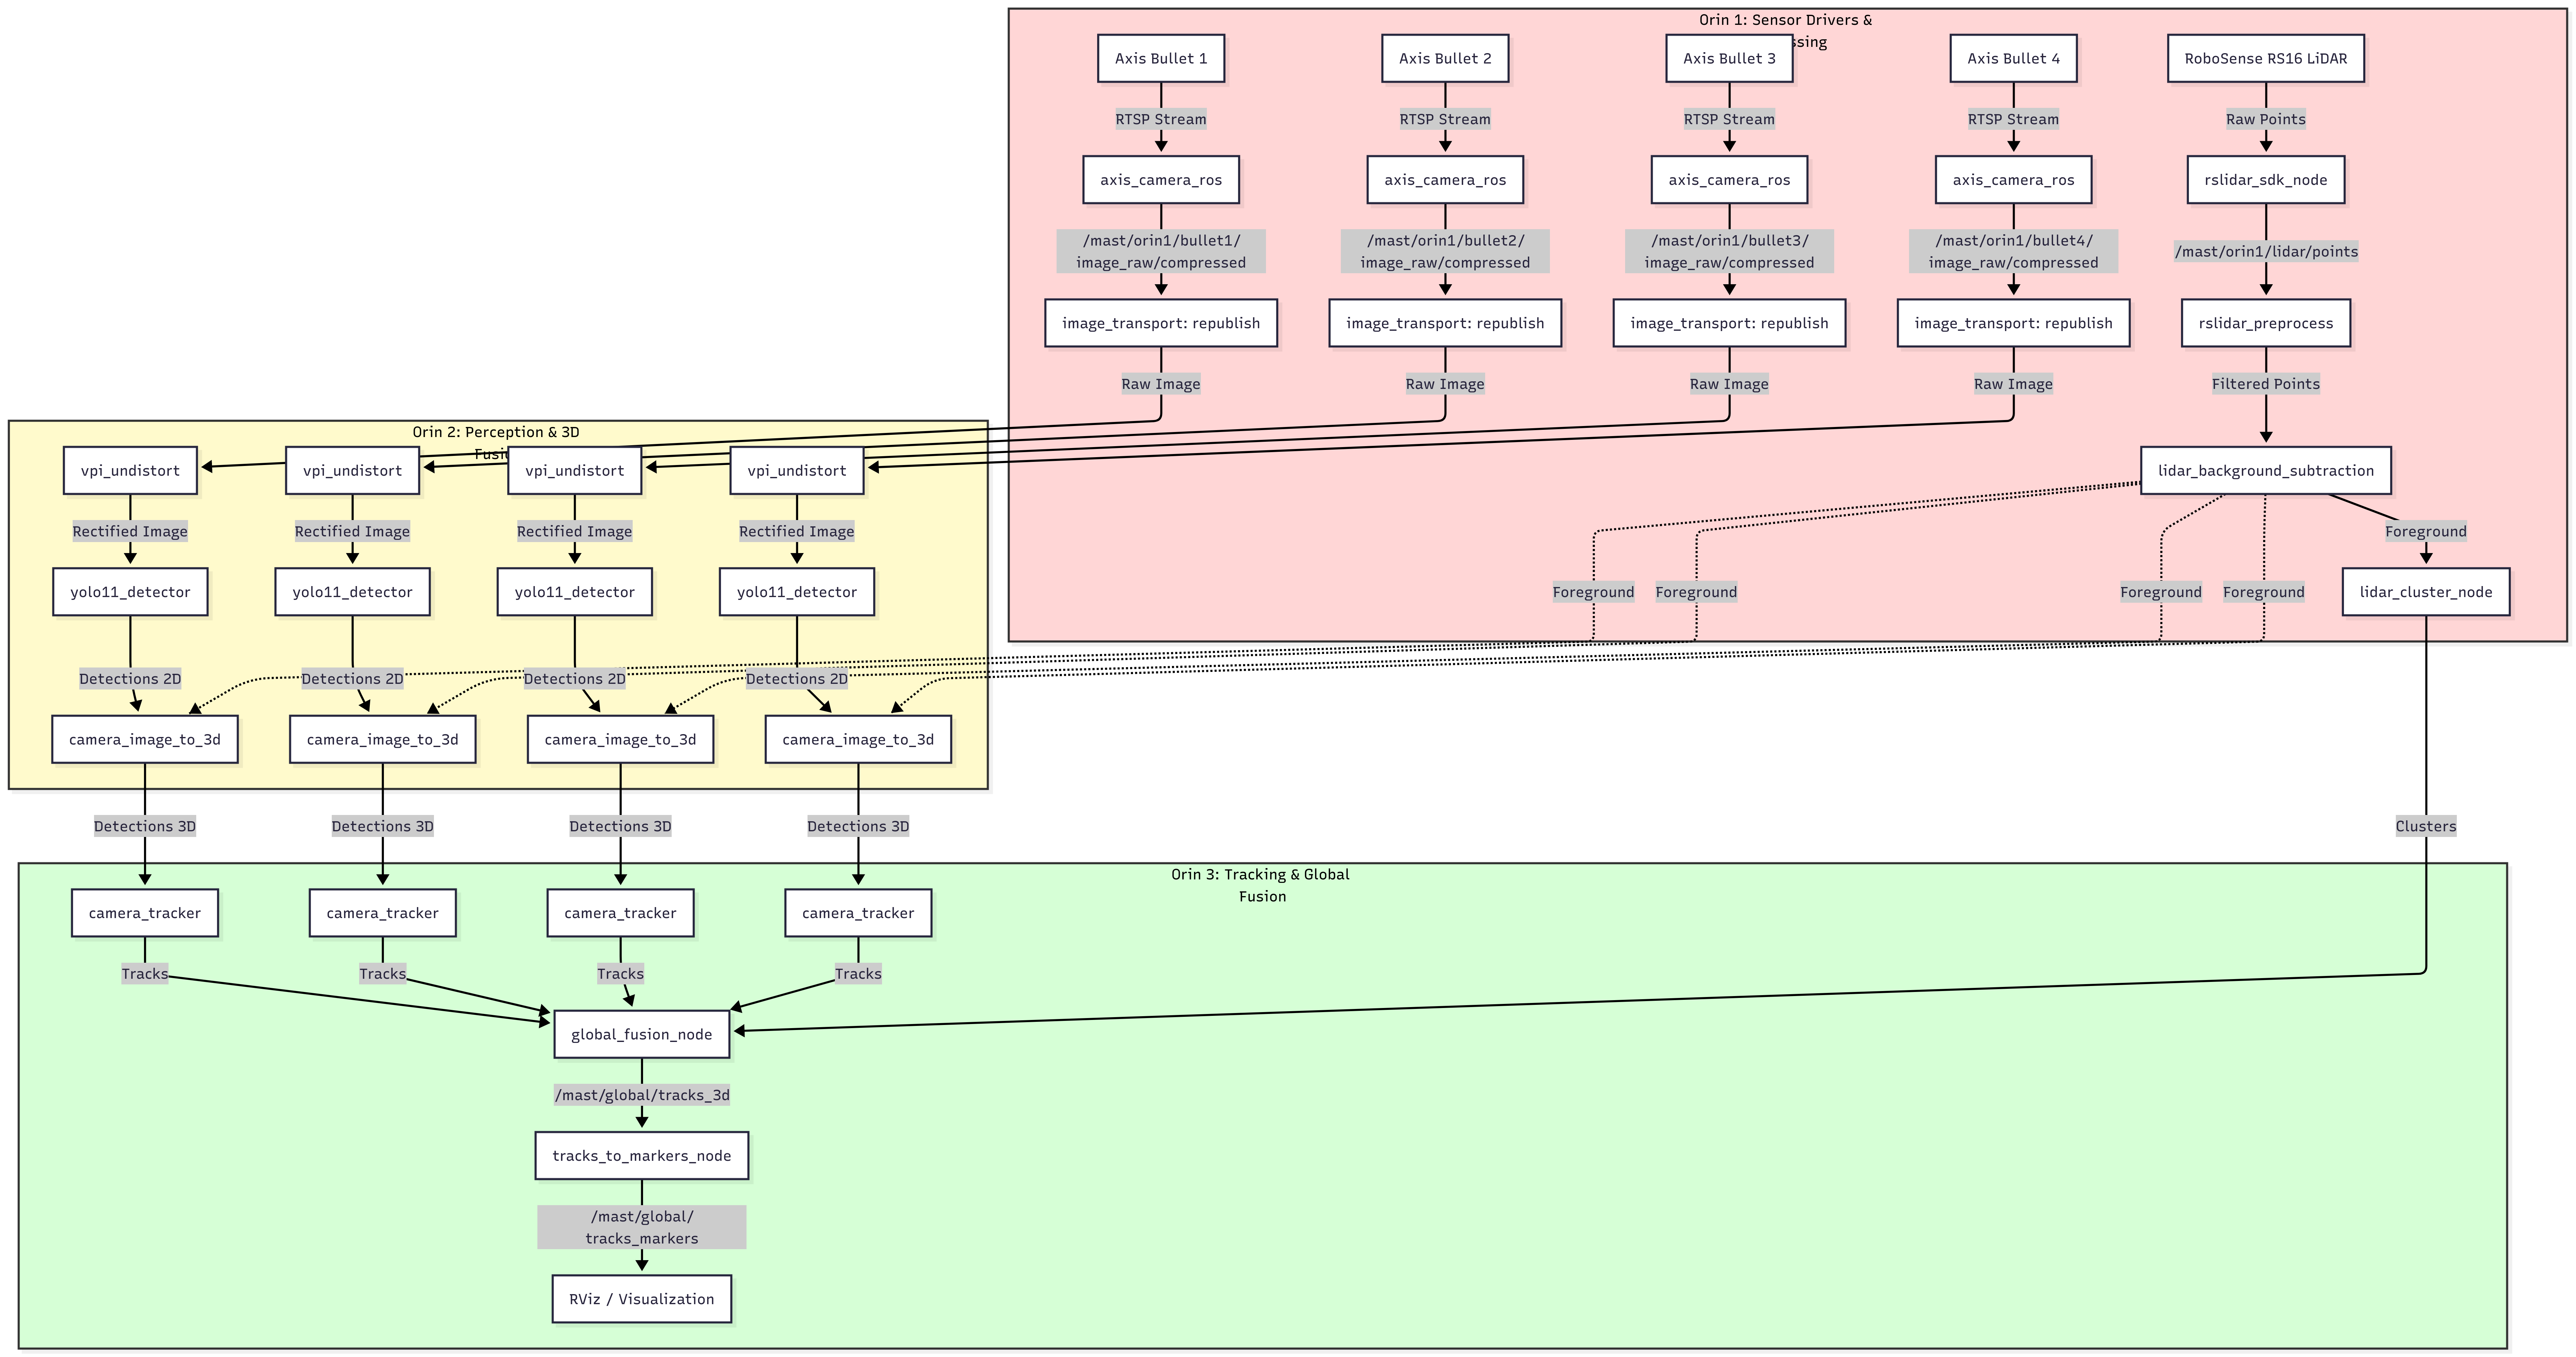
\includegraphics[width=\textwidth]{mermaid-ai-diagram-2026-01-31-205754.png}
    \caption[System Pipeline]{Complete perception pipeline across distributed Jetson Orin devices (System Diagram).}
    \label{fig:pipeline}
\end{figure}

The following system diagrams and component breakdowns illustrate the end-to-end data flow through the distributed cluster.

\subsection{Orin~1 -- Sensor Drivers and Preprocessing}
Jetson Orin~1 is responsible for all sensor-facing components and low-level preprocessing tasks. The following processing steps are executed on this device:
\begin{itemize}
    \item Axis network cameras stream video data via RTSP.
    \item The \texttt{axis\_camera\_ros} package acquires the streams and publishes compressed image topics.
    \item Image republishing nodes convert compressed streams into raw image topics for downstream processing.
    \item The LiDAR driver receives UDP packets and publishes raw point cloud data.
    \item LiDAR preprocessing and background subtraction modules filter static structures and noise.
    \item LiDAR clustering extracts object-level point cloud clusters for higher-level perception.
\end{itemize}

\section{ROS Parameters and Configuration}
The system relies on a centralized parameter server approach using ROS~2 launch files. Key parameters that govern the system behavior include:
\begin{itemize}
    \item \textbf{Global Network Parameters:}
    \begin{itemize}
        \item \texttt{ROS\_DOMAIN\_ID = 0}: Ensures all nodes communicate on the same DDS domain.
        \item \texttt{use\_sim\_time = false}: Set to false for live operation, using PTP-aligned system clocks.
    \end{itemize}
    \item \textbf{Camera Parameters:}
    \begin{itemize}
        \item \texttt{width}: 1920, \texttt{height}: 1080 (Resolution)
        \item \texttt{fps}: 30 (Frame Rate)
        \item \texttt{camera\_info\_url}: \\ \texttt{package://mobile\_mast/config/camera\_info/\$\{name\}.yaml}
    \end{itemize}
    \item \textbf{LiDAR Parameters:}
    \begin{itemize}
        \item \texttt{msop\_port}: 6699 (Data Packet Port)
        \item \texttt{difop\_port}: 7788 (Device Info Packet Port)
        \item \texttt{frame\_id}: \texttt{rslidar}
    \end{itemize}
\end{itemize}


\section{System Inputs and Outputs}

\subsection{Inputs}
\begin{itemize}
    \item Camera image streams (\texttt{/image\_raw})
    \item LiDAR point clouds (\texttt{/lidar/points})
    \item Camera calibration data (\texttt{CameraInfo})
    \item Configuration parameters
\end{itemize}

\subsection{Outputs}
\begin{itemize}
    \item Rectified images (\texttt{/image\_rect})
    \item 2D object detections
    \item 3D object detections
    \item Tracked object states
    \item Global fused tracks
    \item RViz visualization markers
    \item Rosbag recordings for offline analysis
\end{itemize}



\section{ROS~2 Nodes, Topics, and Data Flow}
The complete perception system is implemented as a collection of modular ROS~2 nodes distributed across three NVIDIA Jetson Orin devices. Each node performs a well-defined task and communicates exclusively through ROS~2 topics, following a publisher--subscriber model. This design ensures modularity, scalability, and ease of debugging.

\subsection{Orin~1 -- Sensor Drivers and Preprocessing Nodes}

\paragraph{axis\_camera\_ros}
\begin{description}[leftmargin=1.3cm,style=nextline]
    \item[Function] Captures live video streams from Axis network cameras using RTSP.
    \item[Publishes] \texttt{/mast/orin1/bulletX/image\_raw/compressed}
    \item[Key parameters] Camera IP address, frame rate, resolution (via ROS parameters in launch file).
\end{description}

\paragraph{image\_transport republish}
\begin{description}[leftmargin=1.3cm,style=nextline]
    \item[Function] Converts compressed camera streams into raw image messages.
    \item[Subscribes] \texttt{/mast/orin1/bulletX/image\_raw/compressed}
    \item[Publishes] \texttt{/mast/orin1/bulletX/image\_raw}
\end{description}

\paragraph{rslidar\_sdk\_node}
\begin{description}[leftmargin=1.3cm,style=nextline]
    \item[Function] Interfaces with the RoboSense RS128 LiDAR sensor and publishes ROS~2 point clouds.
    \item[Publishes] \texttt{/mast/orin1/lidar/points} (\texttt{sensor\_msgs/PointCloud2})
    \item[Configuration] Sensor model YAML, channel calibration CSV, network parameters (IP/port).
\end{description}

\paragraph{rslidar\_preprocess}
\begin{description}[leftmargin=1.3cm,style=nextline]
    \item[Function] Filters raw LiDAR point clouds (range filtering, ground removal, noise suppression).
    \item[Subscribes] \texttt{/mast/orin1/lidar/points}
    \item[Publishes] \texttt{/mast/orin1/lidar/points\_filtered}
\end{description}

\paragraph{lidar\_background\_subtraction}
\begin{description}[leftmargin=1.3cm,style=nextline]
    \item[Function] Separates static background from dynamic foreground points.
    \item[Subscribes] \texttt{/mast/orin1/lidar/points\_filtered}
    \item[Publishes] \texttt{/mast/orin1/lidar/foreground}
    \item[Configuration] CSV/YAML (background thresholds, temporal window parameters).
\end{description}

\paragraph{lidar\_cluster\_node}
\begin{description}[leftmargin=1.3cm,style=nextline]
    \item[Function] Groups foreground points into object clusters (Euclidean clustering).
    \item[Subscribes] \texttt{/mast/orin1/lidar/foreground}
    \item[Publishes] \texttt{/mast/orin1/lidar/clusters}
\end{description}

\subsection[Orin 2 Vision]{Orin~2 -- Vision and 2D--3D Association}

\paragraph{vpi\_undistort\_node}
\begin{description}[leftmargin=1.3cm,style=nextline]
    \item[Function] Corrects lens distortion using NVIDIA VPI.
    \item[Subscribes] \texttt{/mast/orin1/bulletX/image\_raw}, \texttt{/mast/orin1/bulletX/camera\_info}
    \item[Publishes] \texttt{/mast/orin1/bulletX/image\_rect}
    \item[Key parameters] Intrinsic matrix, distortion coefficients, backend (CUDA/VIC).
    \item[Configuration] Uses calibration CSV files located in \texttt{/config/calibration/}.
\end{description}

\paragraph{yolo\_detector\_node}
\begin{description}[leftmargin=1.3cm,style=nextline]
    \item[Function] Performs object detection on rectified images using YOLO/TensorRT.
    \item[Subscribes] \texttt{/mast/orin1/bulletX/image\_rect}
    \item[Publishes] \texttt{/mast/orin1/bulletX/detections\_2d}
\end{description}

\paragraph{camera\_image\_to\_3d}
\begin{description}[leftmargin=1.3cm,style=nextline]
    \item[Function] Projects 2D detections into 3D and associates them with LiDAR clusters.
    \item[Subscribes] \texttt{/mast/orin1/bulletX/detections\_2d}, \texttt{/mast/orin1/lidar/clusters}
    \item[Publishes] \texttt{/mast/orin1/bulletX/detections\_3d}
    \item[Configuration] Camera--LiDAR extrinsic calibration (CSV).
\end{description}

\subsection{Orin~3 -- Tracking, Fusion, and Visualization Nodes}

\paragraph{camera\_tracker\_node}
\begin{description}[leftmargin=1.3cm,style=nextline]
    \item[Function] Tracks detected objects over time using 3D detections.
    \item[Subscribes] \texttt{/mast/orin1/bulletX/detections\_3d}
    \item[Publishes] \texttt{/mast/orin1/bulletX/tracks\_3d}
\end{description}

\paragraph{global\_fusion\_node}
\begin{description}[leftmargin=1.3cm,style=nextline]
    \item[Function] Merges camera tracks and LiDAR clusters to produce globally consistent tracks.
    \item[Subscribes] Camera tracks, LiDAR clusters
    \item[Publishes] \texttt{/mast/global/tracks\_3d}
\end{description}

\paragraph{tracks\_to\_markers\_node}
\begin{description}[leftmargin=1.3cm,style=nextline]
    \item[Function] Converts fused tracks into RViz markers for visualization.
    \item[Subscribes] \texttt{/mast/global/tracks\_3d}
    \item[Publishes] \texttt{/mast/global/tracks\_markers}
\end{description}

\section{Configuration Files and CSV Usage}
Several nodes rely on external configuration files to ensure flexibility and accuracy. Table~\ref{tab:config-files} summarizes the main configuration dependencies.

\begin{table}[H]
\centering
\caption[Configuration files]{Configuration files used by key nodes.}
\label{tab:config-files}
\begin{tabularx}{\textwidth}{@{}l l X@{}}
\toprule
\textbf{Node / Module} & \textbf{File type} & \textbf{Purpose} \\
\midrule
VPI undistortion & YAML / CSV & Camera intrinsics and distortion coefficients \\
LiDAR driver & YAML / CSV & Sensor model and channel/angle calibration \\
2D--3D projection & YAML / CSV & Camera--LiDAR extrinsics and transforms \\
Tracking nodes & YAML & Filter parameters and thresholds \\
\bottomrule
\end{tabularx}
\end{table}

\section{End-to-End Data Flow Summary}
\begin{itemize}
    \item Sensors generate raw camera images and LiDAR point clouds.
    \item Data is preprocessed and filtered on Orin~1.
    \item Images are undistorted and objects detected on Orin~2.
    \item 2D detections are projected into 3D space.
    \item Objects are tracked and fused on Orin~3.
    \item Results are visualized in RViz and recorded using rosbag.
\end{itemize}

% =========================================================
% 3 LiDAR Perception Pipeline
% =========================================================
\chapter{LiDAR Implementation}
% --- PREAMBLE SUGGESTIONS (Add these to the top of your main.tex if not present) ---
% \usepackage{listings}
% \usepackage{xcolor}
% \usepackage{hyperref}

% \lstset{


\section[LiDAR Integration]{LiDAR Hardware Integration and Drivers}


The implementation phase followed a rigorous two-stage integration strategy. Before deploying the software to the embedded system, I first validated the RoboSense Ruby Plus (128-beam) hardware using a standard Linux-based laptop. This ``bench test'' phase allowed me to isolate potential hardware defects and verify the driver configuration in a controlled environment before migrating the computation to the final NVIDIA Jetson Orin compute unit.

\subsection{Phase 1: Initial Hardware Verification (Linux Laptop)}
The first step involved interfacing the LiDAR hardware directly with my personal Linux workstation to verify the sensor's functionality and establish a baseline for network communication.

\textbf{Network Interface Configuration:} Since the Ruby Plus generates a massive volume of data points, establishing a stable Ethernet connection was critical. I physically connected the LiDAR’s interface box to the laptop’s Ethernet port. To enable communication, I manually configured the laptop's wired network profile to operate on the same static subnet as the sensor.

\begin{itemize}
    \item \textbf{LiDAR IP:} Verified as \texttt{192.168.6.60}.
    \item \textbf{Laptop IP:} I assigned the static address \texttt{192.168.6.50} to the laptop to act as the temporary host.
\end{itemize}

I performed a connectivity check using the \texttt{ping} command to ensure the physical link was stable.

\begin{figure}[ht!]
    \centering
    \begin{verbatim}
ping 192.168.6.60
    \end{verbatim}
    \caption{Connectivity check with LiDAR}
    \label{fig:ping_check}
\end{figure}

The response confirmed a low-latency connection ($< 1$ms), validating the physical cabling and power supply.

\textbf{Driver Setup and Visualization:} With connectivity established, I navigated to the official RoboSense website and downloaded the \texttt{rslidar\_sdk} driver package tailored for the Ruby Plus series. I created a local ROS~2 workspace on the laptop, installed the necessary build dependencies, \texttt{yaml}), and compiled the driver.

To confirm the sensor was scanning correctly, I launched the driver node and opened RViz2 on the laptop. The visualization of the point cloud confirmed that the sensor’s lasers were firing correctly and the internal motors were spinning at the desired RPM.

\subsection{Phase 2: Migration to NVIDIA Jetson Orin}
Following the successful validation on the laptop, I proceeded to migrate the software stack to the final deployment target: the NVIDIA Jetson Orin. This transition involved replicating the environment and offloading the heavy computational tasks to the Orin’s ARM-based architecture.

\textbf{Dependency Management on Orin:} I accessed the Jetson Orin via SSH and prepared the Linux environment. I manually installed the prerequisite libraries required for packet capturing, ensuring they matched the versions used during the laptop test to prevent compatibility issues:

\begin{itemize}
    
    \item \texttt{yaml file}: Essential for parsing the driver configuration files.
\end{itemize}

\textbf{Final Network Configuration:} I configured the Orin’s primary network interface to the static IP \texttt{192.168.6.1}, establishing it as the permanent gateway for the sensor suite.

% The [H] forces the image to stay right here
\begin{figure}[H]
    \centering
    \includegraphics[width=0.8\linewidth]{AI_Mobile_Perception_Professional_60p_final/figures/LiDAR Point cloud Visualization.jpeg}
    \caption{LiDAR Point Cloud Visualization Rviz2}
    \label{fig:lidar_viz}
\end{figure}

\subsection{Driver Configuration and Parameter Tuning}
The default driver configuration provided by the manufacturer is generic. To ensure optimal performance on the Orin, I explicitly tailored the \texttt{config.yaml} file located within the driver package.

\textbf{Key Configuration Changes:}
\begin{itemize}
    \item \textbf{LiDAR Type Definition:} I modified the \texttt{lidar\_type} parameter to \texttt{RS128}. This was a critical step; without this specific definition, the driver would misinterpret the data structure of the 128-beam sensor, resulting in corrupted point clouds.
    
    \item \textbf{Port Mapping:} I edited the MSOP (Data) and DIFOP (Device Info) ports to match the values \texttt{6699} and \texttt{7788}, ensuring the driver listened on the correct UDP channels mapped during the network setup.
    
    \item \textbf{Coordinate Frame:} I defined the \texttt{frame\_id} as \texttt{rslidar} to establish the root of our transformation tree.
\end{itemize}

\subsection{Node Creation and System Validation}
To finalize the integration, I created a dedicated launch file for the LiDAR node on the Orin. This node is responsible for ingesting the raw UDP packets and converting them into standard \texttt{sensor\_msgs/PointCloud2} messages for the rest of the ROS~2 system.

\textbf{Verification Steps:} Upon launching the node, I inspected the active ROS~2 topics to verify the data flow was being computed correctly by the Orin.

\begin{figure}[ht!]
    \centering
    \begin{verbatim}
ros2 topic list
ros2 topic hz /rslidar_points
    \end{verbatim}
    \caption{Verifying ROS~2 Topics and Frequency}
\end{figure}

\section{Summary}
This chapter presented the complete hardware integration and driver deployment for the LiDAR sensor. The migration of the software stack from the development laptop to the NVIDIA Jetson Orin was validated through visual confirmation in RViz, which showed the point cloud perfectly aligned with the sensor's physical environment.

While the physical integration and data streaming were successfully established, initial frequency checks revealed a significant challenge: the massive data throughput of the 128-beam sensor caused instability, preventing the system from maintaining a stable 10Hz output. The specific middleware optimizations and methodology required to resolve this bottleneck are detailed in the upcoming chapter. With the foundational hardware interface now complete, the system is prepared for the subsequent stages of the perception pipeline including preprocessing, background subtraction, and clustering to transform raw measurements into reliable object-level representations for the mobile mast application.


\section{LiDAR Time Synchronization}


Precise temporal synchronization is a fundamental requirement for multi-sensor fusion systems. In a dynamic environment, even minor timing discrepancies between the LiDAR (10 Hz) and camera (30 Hz) streams can lead to significant alignment errors (``ghosting'') when the vehicle or objects are in motion. This chapter details the engineering challenges faced in synchronizing the RoboSense Ruby Plus sensor and the transition from a hardware-based GNSS solution to a robust network-based Precision Time Protocol (PTP) architecture.

\subsection{Problem Statement: The Need for Microsecond Accuracy}
The perception system operates on a heterogeneous sensor suite. Without a unified time reference, the fusion algorithm would attempt to project 3D points onto 2D images captured at different moments in time. To mitigate this, the system requires a shared clock source (Grandmaster) that synchronizes all sensor timestamps to Universal Coordinated Time (UTC) with microsecond-level precision.

\subsection{Initial Approach: Hardware GNSS/PPS Synchronization}
Our initial design utilized a \textbf{Garmin GPS 18x LVC} receiver for hardware synchronization. This device provides two distinct signals required by the LiDAR:
\begin{enumerate}
    \item \textbf{\$GPRMC (NMEA):} A serial data stream providing the absolute UTC time.
    \item \textbf{PPS (Pulse Per Second):} A high-precision electrical pulse marking the exact start of a second.
\end{enumerate}

\subsubsection{Diagnostic Engineering: The Baud Rate Mismatch}
The GPS unit was wired to the RoboSense Interface Box, but initial tests showed an ``Unlocked'' status. To diagnose this, I developed a \textbf{temporary diagnostic node} in ROS~2 (\texttt{serial\_debugger\_node}) to analyze the raw NMEA data.
By iterating through standard baud rates (4800, 9600, 115200) within the node, I successfully decoded the NMEA sentences at 4800 bps. However, the RoboSense LiDAR firmware is hard-coded to expect NMEA data at 9600 bps. This mismatch meant the LiDAR was interpreting the valid 4800 bps GPS data as noise, preventing synchronization.

\textbf{Resolution Attempt:}
To rectify this, I interfaced the GPS with a separate utility and reprogrammed its non-volatile memory to force a 9600 bps output. While this successfully allowed the LiDAR to parse the NMEA packets, the synchronization remained intermittent due to electrical noise in the wiring harness. Consequently, this hardware-heavy approach was deemed too unreliable for the final operational environment.

\subsection[Final Solution: PTP]{Final Solution: PTP (IEEE 1588)}
To overcome the limitations of the physical GPS connection, the system was migrated to a network-based synchronization strategy using the \textbf{Precision Time Protocol (PTP)}, defined by the IEEE 1588 standard. Unlike the Network Time Protocol (NTP), which offers millisecond-level accuracy, PTP utilizes hardware timestamping at the Ethernet MAC layer to achieve sub-microsecond synchronization.

\subsubsection{Architecture Implementation}
In this architecture, the NVIDIA Jetson Orin serves as the \textbf{PTP Grandmaster Clock}, broadcasting high-precision time packets to all connected sensors over the Ethernet network.

\subsubsection{Software Configuration}
The implementation required configuring the Linux PTP stack on the compute unit and adjusting the LiDAR's internal firmware settings.

\textbf{1. Master Clock Configuration (Jetson Orin):}
I installed the \texttt{linuxptp} package and configured the \texttt{ptp4l} daemon to operate in master mode on the dedicated sensor interface (\texttt{eth0}). The configuration ensured the Orin prioritized its own system clock as the authoritative time source.

\begin{lstlisting}[language=bash, caption={Launching PTP4L in Master Mode}]
# Run PTP4L on interface eth0 in master-only mode
sudo ptp4l -i eth0 -m -4
\end{lstlisting}

\textbf{2. Slave Configuration (RoboSense LiDAR):}
Accessing the sensor's web configuration portal, I modified the \textit{Time Sync Source} parameter from ``GPS'' to ``PTP/1588''.

\subsection{Results and Validation}
Upon applying the PTP configuration, the synchronization stability was verified using the sensor's telemetry feedback.
\begin{itemize}
    \item \textbf{Lock Time:} The sensor achieves a ``Locked'' state within 30 seconds of boot.
    \item \textbf{Drift:} The offset between the LiDAR timestamp and the Orin system time was measured at $< 5$ microseconds.
\end{itemize}

This transition to PTP eliminated the need for external satellite visibility, allowing for reliable sensor fusion development in both indoor laboratory settings and outdoor deployment.

% =========================================================
% 4 Camera Perception and Time Synchronization Pipeline
% =========================================================
\chapter[Camera Perception Pipeline]{Camera Perception and \\ Time Synchronization Pipeline}

\section{Axis Camera System Overview}
Camera sensors play a critical role in perception systems by providing dense visual and semantic information about the environment. In the proposed system, Axis network cameras are used to capture continuous video streams of the surroundings from elevated viewpoints on a mobile mast. These cameras provide high-resolution imagery suitable for object detection, tracking, and multi-sensor fusion.

Unlike range sensors, cameras do not directly measure depth. Their effectiveness in multi-sensor perception systems therefore depends on accurate calibration, geometric correction, and precise temporal alignment with LiDAR measurements.

\section{Camera Data Acquisition}
\subsection{Axis Camera Hardware}
The Axis cameras used in this system are IP-based surveillance cameras equipped with wide-angle lenses. They support:
\begin{itemize}
    \item Network-based streaming
    \item Hardware timestamping
    \item High frame rate video capture
\end{itemize}
The cameras are mounted rigidly to maintain stable extrinsic relationships with the LiDAR sensor.

\subsection{RTSP Streaming}
Each Axis camera transmits video using RTSP protocols. Frames are encoded using standard video compression techniques and transmitted over Ethernet. Let $I_c(t)$ denote the camera image captured at time $t$. The camera produces a sequence:
\begin{equation}
\{ I_c(t_1), I_c(t_2), \dots, I_c(t_n) \},
\end{equation}
where $t_i$ corresponds to camera clock timestamps.

\subsection{axis\_camera\_ros Node}
\textbf{Node name:} \texttt{axis\_camera\_ros}

\textbf{Function:} Captures network video streams and publishes them as ROS~2 image messages.

\textbf{Published topics:}
\begin{itemize}
    \item \texttt{/mast/orin1/bulletX/image\_raw/compressed}
    \item \texttt{/mast/orin1/bulletX/image\_raw}
\end{itemize}

\section{Camera Image Transport and Processing}
\subsection{Compressed Image Transport}
Compressed image transport significantly reduces bandwidth usage, which is crucial for transmitting multiple high-definition streams over the network. The \texttt{axis\_camera\_ros} node publishes images in JPEG format:
\begin{itemize}
    \item \textbf{Topic:} \texttt{/mast/orin1/bulletX/image\_raw/compressed}
    \item \textbf{Format:} \texttt{jpeg}
\end{itemize}
These compressed images are efficient for monitoring but unsuitable for processing (Undistortion/YOLO) which requires raw pixel data.

\subsection{Raw Image Republishing}
To prepare images for processing, the \texttt{image\_transport} republish node decodes the compressed streams into raw \texttt{sensor\_msgs/Image} messages. This step typically runs on the processing unit (Orin 2) to keep the raw data local to the inference engine.
\begin{equation}
I_c^{\mathrm{raw}}(t) = \mathrm{Decode}\bigl(I_c^{\mathrm{comp}}(t)\bigr).
\end{equation}

\section{Camera Time Synchronization}
Accurate temporal alignment between camera images and LiDAR point clouds is essential for correct spatial association.

\subsection{LiDAR Time Reference (GPS Time)}
The LiDAR sensor operates on a GPS-disciplined clock, producing timestamps in a global time reference $T_{\mathrm{GPS}}$. LiDAR point clouds are stamped as $P_L(T_{\mathrm{GPS}})$ and used as the system master reference.

\subsection{Camera Time Alignment Strategy}
Camera timestamps $T_c$ are aligned to the LiDAR reference using an offset correction:
\begin{equation}
T_c^{\mathrm{aligned}} = T_c + \Delta T,
\end{equation}
where $\Delta T$ is the estimated clock offset between the camera and LiDAR clocks.

\subsection{Precision Time Protocol (PTP) Integration}
To minimize clock drift and offset, Precision Time Protocol (PTP) is used. The clock offset can be estimated as:
\begin{equation}
\Delta T = \frac{(t_2 - t_1) + (t_3 - t_4)}{2},
\end{equation}
where $t_1,t_2,t_3,t_4$ are PTP message timestamps.

\section{Camera Image Undistortion (NVIDIA VPI)}
Wide-angle lenses introduce non-linear distortions that affect geometric accuracy. To ensure reliable 2D--3D association, the system performs GPU-accelerated undistortion using NVIDIA VPI.

\subsection{Lens Distortion Model}
The pinhole camera model with radial and tangential distortion is used:
\begin{equation}
\begin{aligned}
x_d &= x_u (1 + k_1 r^2 + k_2 r^4 + k_3 r^6) + 2p_1 x_u y_u + p_2(r^2 + 2x_u^2), \\
y_d &= y_u (1 + k_1 r^2 + k_2 r^4 + k_3 r^6) + p_1(r^2 + 2y_u^2) + 2p_2 x_u y_u,
\end{aligned}
\end{equation}
where $r^2 = x_u^2 + y_u^2$, $(x_u,y_u)$ are undistorted normalized coordinates, and $(x_d,y_d)$ are distorted coordinates.

\subsection{GPU-Accelerated Undistortion}
VPI precomputes a \emph{WarpMap} that defines a pixel-wise mapping between rectified and distorted image coordinates. This mapping is then applied efficiently on the GPU for each frame to produce a rectified image topic:
\begin{itemize}
    \item Input: \texttt{/mast/orin1/bulletX/image\_raw}
    \item Output: \texttt{/mast/orin1/bulletX/image\_rect}
\end{itemize}

\subsection{Why NVIDIA VPI Is Used}
The choice of NVIDIA Vision Programming Interface (VPI) for image undistortion is driven by the need for high-throughput and low-latency processing in a multi-camera setup. Traditional CPU-based undistortion methods, such as those provided by standard OpenCV implementations, often become a bottleneck when processing multiple high-resolution streams (e.g., 1080p or 4K) at 30 FPS. 

VPI provides several critical advantages:
\begin{itemize}
    \item \textbf{Hardware Acceleration:} VPI leverages the dedicated hardware engines on the Jetson Orin, including the Programmable Vision Accelerator (PVA) and the Video Image Compositor (VIC), in addition to the GPU (via CUDA). This offloading ensures that the main GPU remains available for deep learning inference (YOLO).
    \item \textbf{Stream-Based API:} VPI's asynchronous stream-based execution model allows for overlapping memory transfers with computation, maximizing hardware utilization.
    \item \textbf{Precomputed Remap Tables:} By precomputing the WarpMap based on the camera intrinsic and distortion parameters, VPI reduces the per-frame overhead to a simple remapping operation, which is highly optimized for the Jetson hardware.
    \item \textbf{Zero-Copy Memory Access:} VPI facilitates efficient memory sharing between different hardware engines and ROS~2 image buffers, minimizing unnecessary data copies.
\end{itemize}

In our implementation, the undistortion node subscribes to the raw image topic, performs the remapping using the CUDA backend for maximum speed, and publishes the rectified image to be used by the YOLO detector. This architecture allows us to maintain a stable frame rate even with heavy computational loads.

\section{Datasets and Data Preparation}
In this project, multiple large-scale public datasets were combined to construct a comprehensive and diverse training set for camera-based object detection in urban traffic environments. The selected datasets cover a wide range of traffic participants, viewpoints, weather conditions, and scene complexities, which is essential for building a robust perception system suitable for real-world deployment.



\subsection{\textbf{Overview of Used Datasets} }
The project integrates several key datasets to cover a broad spectrum of traffic environments and perspectives. For infrastructure-based viewpoints, the TUMTraf A9 R1 Highway Dataset was incorporated, utilizing three distinct scenarios to capture varying traffic densities. To improve the detector’s performance under fixed-camera and mobile mast perspectives, the UA-DETRAC and VisDrone datasets were also included. In particular, VisDrone was selected to address challenging top-down viewpoints and significant object scale variations. 

The training set's diversity was further expanded by leveraging BDD100K for varied weather conditions and Cityscapes for high-quality European urban scenes. To ensure effective recognition of vulnerable road users, the EuroCity Persons dataset was utilized for its extensive pedestrian and cyclist labels. Additionally, RSUD20K was integrated for its dense object annotations, while the RGB component of the R-LiViT RGB-T Dataset was used to improve robustness under shifting illumination. By combining these heterogeneous sources, the resulting dataset provides a comprehensive foundation for complex, real-world traffic monitoring.
An overview of the datasets and their primary contributions is provided in Table~\ref{tab:datasets}.

\begin{table}[H]
\centering
\caption[Dataset Summary]{Summary of datasets used for training and evaluation}
\label{tab:datasets}
\begin{tabularx}{\textwidth}{l l >{\raggedright\arraybackslash}X}
\hline
\textbf{Dataset} & \textbf{Viewpoint / Scenario} & \textbf{Primary Contribution} \\
\hline
TUMTraf A9 Highway & Infrastructure-based, highway & Multi-scenario traffic density and long-range detection \\
UA-DETRAC & Fixed traffic cameras & Vehicle detection under surveillance-style viewpoints \\
VisDrone & Aerial / top-down & Scale variation and top-down object detection \\
BDD100K & On-board camera & Weather, illumination, and scene diversity \\
Cityscapes & Urban, European cities & High-quality annotations for urban traffic scenes \\
EuroCity Persons & Urban street-level & Pedestrian and cyclist detection (VRUs) \\
RSUD20K & Dense traffic scenes & High object density and cluttered environments \\
R-LiViT (RGB only) & Multi-condition RGB & Robustness to illumination changes \\
\hline
\end{tabularx}
\end{table}
Additionally, smaller auxiliary datasets focusing on specific object categories (e.g., motorcycles and e-scooters) were incorporated to address class imbalance issues observed in the initial training data. These datasets were treated as supplementary sources and merged carefully into the main training set.

\subsection{Dataset Integration}
Due to the heterogeneous nature of the selected datasets, a unified data integration strategy was required to prepare the data for training. Thus, all datasets were converted into a common YOLO-compatible format, a process that involved harmonizing class definitions across diverse sources and mapping dataset-specific labels to a unified class index set. In addition, unsupported or irrelevant classes were removed to ensure consistency across the combined dataset. Special care was taken to maintain a correct correspondence between images and their labels throughout the preprocessing stage, as this is essential for reliable training. After completing these preprocessing steps, all datasets were merged into a single unified dataset, referred to as \textit{global\_yolo}. This combined dataset was then used as the main training set for the object detection model.

\subsection{Annotation Formats and Conversion}
The original datasets utilized a variety of annotation formats, ranging from YOLO text and PASCAL VOC XML to various dataset-specific schemas. To standardize the training pipeline, all annotations were converted into a uniform YOLO format featuring normalized bounding box coordinates. This transformation was executed using custom conversion scripts designed to parse the original annotation files, validate bounding box integrity, and generate consistent label files across the entire integrated dataset. 

The conversion process ensured that each image had exactly one corresponding label file, invalid or empty annotations were removed and bounding boxes were correctly normalized based on image resolution.

\subsection{Training and Validation Split}
Training and validation splits were preserved according to the original dataset definitions whenever possible to avoid data leakage.  Therefore, all datasets were combined at the training level, while validation was performed on a fixed and consistent validation set. This ensured fair performance comparison across different training configurations and prevented overfitting to newly added data sources.

\subsection{Final Dataset Statistics}
Following the completion of preprocessing and integration, the final dataset comprises 201,354 images and an equivalent number of label files, representing a total of 1,293,541 annotated object instances. This unified training set contains seven distinct object classes, with the following class-to-index mapping:

\begin{itemize}
    \item 0: person
    \item 1: bicycle
    \item 2: motorcycle
    \item 3: car
    \item 4: bus
    \item 5: truck
    \item 6: e-scooter
\end{itemize}
By incorporating over 1.2 million instances, the dataset provides a high-density data foundation that allows the model to learn robust features across diverse urban environments while ensuring a large-scale representation of both dominant and minority vehicle classes.

\subsection{Dataset Configuration}
All datasets were accessed through a single unified dataset configuration file, named \texttt{global\_yolo.yaml}. This file specifies the paths to the training and validation images, as well as the unified list of object classes used during training. Using a single configuration file made it easier to manage the datasets and allowed new data to be added with minimal changes to the overall setup.

This final dataset configuration step provided a solid foundation for the deep learning–based object detection approach described in the following section.


\section{Deep Learning-Based Object Detection}
This section describes the deep learning–based object detection component of the camera perception pipeline. The objective is to detect relevant road users in the 2D image plane and to output class-labeled bounding boxes. These detections are subsequently consumed by downstream modules (e.g., global tracking and multi-sensor fusion) as structured semantic observations.

A YOLOv11-based single-stage detector was selected due to its favorable accuracy-latency trade-off and its practicality for real-time use on GPU-equipped systems. In the conducted experiments, the YOLOv11s model variant was employed as a compact baseline that balances detection performance with computational constraints.

\subsection{Detection Output and Interface}
For each RGB image frame, the detector produces a set of detections. Each detection contains a class label (from the predefined traffic-related categories), a confidence score indicating the model’s certainty and a 2D bounding box in pixel coordinates (top-left and bottom-right corners).

The detector therefore performs both classification (“what object is present?”) and localization (“where is it in the image?”). The output is formatted in a standard object-detection representation that enables straightforward integration into later perception stages, where detections can be associated over time and across sensors.




\subsection[Training Configuration]{Training Configuration and Practical Considerations}

The final training run was configured to improve detection quality on a diverse merged dataset (\textit{global\_yolo}), which includes multiple traffic datasets. For improved small-object detection and more robust localization, the input resolution was increased from the earlier 640 setting to imgsz = 960.

A representative training configuration is summarized below (as described in the experiment logs):

\begin{itemize}
    \item Model initialization: trained starting from a previously obtained best checkpoint (transfer learning).
    \item Input size: 960 × 960
    \item Batch size: 8
    \item Early stopping: enabled (patience = 10) to prevent unnecessary training once validation performance saturates.
    \item Caching: caching-to-RAM was attempted; however, system RAM was insufficient for full caching, and partial/no caching was applied automatically (as indicated by runtime warnings).
    \item Label integrity checks: duplicate labels were detected in parts of the dataset and automatically removed by the training pipeline. This indicates that label sanitation was handled during training, reducing annotation noise.
\end{itemize}

 
\subsection{Fine-Tuning and Class-Specific Improvements}
Initial training experiments revealed that certain minority classes (most notably motorcycles and e-scooters) exhibited lower recall compared to dominant vehicle classes such as cars and buses. This behavior is common in traffic datasets due to inherent class imbalance. To address this issue, targeted fine-tuning for both motorcycle and e-scooter instances was conducted by incorporating additional class-specific training samples and selectively freezing early network layers. Specifically, additional datasets focused on these minority categories were integrated into the training set. Subsequently, training was resumed from pre-trained weights instead of starting from scratch, and training schedules were adjusted to allow the model to adapt to the newly introduced data without degrading overall performance. These steps resulted in a measurable improvement in detection stability for motorcycles and e-scooters while preserving strong performance for other classes.

\subsection{Quantitative Results and Interpretation (Fatih)}
Model performance was evaluated using standard object detection metrics:

\begin{itemize}
    \item Precision (P): fraction of predicted boxes that are correct.
    \item Recall (R): fraction of ground-truth objects that are detected.
    \item mAP@0.50: mean Average Precision at IoU threshold 0.50 (moderate localization requirement).
    \item mAP@0.50:0.95: mAP averaged over stricter IoU thresholds (more demanding localization quality).
\end{itemize}
The aggregated validation metrics for the final YOLOv11s run are presented in Table 4.7.1.

\begin{table}[H]
\centering
\caption[Validation metrics]{Validation metrics of the final YOLOv11s model trained with imgsz=960.}
\label{tab:values}
\begin{tabular}{lll}
\hline
\textbf{Metric} & \textbf{Value} \\
\hline
Precision & 0.48 \\
Recall & 0.54 \\
mAP@0.50 & 0.48 \\
mAP@0.50:0.95 & 0.36 \\
\hline
\end{tabular}
\end{table}
The validation results  indicate that the detector achieves a moderate overall accuracy, with recall being slightly higher than precision. This suggests that the model is capable of detecting a large portion of objects, while still producing a non-negligible number of false positives. The gap between mAP@0.50 and mAP@0.50:0.95 further suggests that localization quality under stricter IoU thresholds remains challenging, which is typical in large-scale multi-source datasets and small-object scenarios. 

\subsection{Precision–Recall and F1 Curve Analysis (Fatih)}
To further analyze the behavior of the trained model across different confidence thresholds, precision–recall (PR), F1-score, precision, and recall curves were examined. These curves provide insight into the trade-off between detection accuracy and completeness and help assess the stability of the model beyond single-point metrics.

\begin{figure}[!htbp]
  \centering
  \begin{subfigure}[t]{0.48\linewidth}
    \centering
    \includegraphics[width=\linewidth]{figures/BoxPR_curve.png}
    \caption{PR curve}
    \label{fig:boxpr}
  \end{subfigure}
  \hfill
  \begin{subfigure}[t]{0.48\linewidth}
    \centering
    \includegraphics[width=\linewidth]{figures/BoxF1_curve.png}
    \caption{F1--confidence curve}
    \label{fig:boxf1}
  \end{subfigure}
  \caption{Confidence-threshold analysis for the trained YOLO detector.}
  \label{fig:pr_f1}
\end{figure}

As shown in Figure~\ref{fig:pr_f1}, the PR curve depicts the inverse relationship between precision and recall, a characteristic behavior in complex object detection tasks. The F1 curve highlights the operating region where precision and recall are balanced, indicating a suitable confidence threshold for deployment. Thus, the observed curves suggest that the detector maintains stable performance across a reasonable range of confidence values, without abrupt degradation in either precision or recall.

Overall, this analysis supports the robustness of the trained model and justifies the selected confidence threshold used during the evaluation and deployment preparation.

\subsection{Analysis of Training Curves (Fatih)}
The training and validation dynamics are summarized in the results plot shown in Figure~\ref{fig:results}, which includes box loss, classification loss, and distribution focal loss, as well as precision, recall, and mAP curves over training epochs.

\begin{figure}[H]
    \centering
    \includegraphics[width=0.90\linewidth]{AI_Mobile_Perception_Professional_60p_final/figures/results.png}
    \caption{Training/validation losses and detection metrics over epochs for the final YOLOv11s run.}
    \label{fig:results}
\end{figure}


Based on the trends observed in Figure~\ref{fig:results} , training losses decrease rapidly during the early epochs and then plateau, indicating fast convergence under transfer learning. Validation mAP reaches its peak relatively early, around the epoch where the best checkpoint is saved, and does not improve significantly afterward, which explains the activation of early stopping. Additionally, the metric curves exhibit noticeable fluctuations, which is expected in heterogeneous datasets composed of multiple sources, where domain shift and class imbalance can lead to noisy validation signals. 


\subsection{Normalized Confusion Matrix (Fatih)}
The normalized confusion matrix shown in Figure~\ref{fig:confusionmatrix} provides insights into which object classes are most frequently confused by the model. Since the matrix is normalized, each column reflects how true instances of a given class are distributed across the predicted classes. 
\begin{figure}[H]
    \centering
    \includegraphics[width=0.90\linewidth]{AI_Mobile_Perception_Professional_60p_final/figures/confusion_matrix_normalized.png}
    \caption{Normalized confusion matrix of the final YOLOv11s model on the validation set.}
    \label{fig:confusionmatrix}
\end{figure}
As observed in  Figure~\ref{fig:confusionmatrix} , misclassifications tend to occur between visually similar categories, which is consistent with typical confusion patterns in the traffic domain. These confusions are most prominent among related classes such as cars and trucks, particularly in scenarios involving occlusion or significant object distance. Furthermore, the presence of a non-trivial distribution in the background row and column highlights persistent challenges related to missed detections and false positives, often triggered by small objects or cluttered scenes. This analysis directly motivates targeted improvements, including the integration of class-specific data and the application of domain-specific fine-tuning to achieve better class balance. 

\subsection{Qualitative Results (Fatih)}
To complement the quantitative evaluation, the predicted detections on validation images were qualitatively inspected. Representative examples comparing model predictions with ground-truth annotations are presented in Figure~\ref{fig:qualitative_comparison}. 


\begin{figure}[H]
    \centering

    \begin{subfigure}[b]{0.9\linewidth}
        \centering
        \includegraphics[width=\linewidth]{AI_Mobile_Perception_Professional_60p_final/figures/val_batch1_pred.jpg}
        \caption{Model predictions on validation images}
    \end{subfigure}

    \vspace{0.4cm}

    \begin{subfigure}[b]{0.9\linewidth}
        \centering
        \includegraphics[width=\linewidth]{AI_Mobile_Perception_Professional_60p_final/figures/val_batch1_labels.jpg}
        \caption{Ground-truth annotations}
    \end{subfigure}

    \caption{Qualitative comparison between model predictions and ground-truth annotations on validation images.}
    \label{fig:qualitative_comparison}
\end{figure}
As shown in Figure~\ref{fig:qualitative_comparison}, the predicted bounding boxes closely match the ground-truth annotations for most traffic participants. The qualitative results indicate that the detector reliably identifies common traffic objects while producing spatially coherent bounding boxes. On the other hand, certain edge cases persist, particularly in scenarios involving strong occlusions or objects appearing at significant distances, where reduced pixel resolution limits detection accuracy.

Detection performance tends to decrease under poor lighting and low-contrast conditions, as important visual features may be hidden. Additionally, class ambiguity remains a contributing factor for visually similar categories, such as bicycles and motorcycles, especially when motion blur or environmental noise complicates the distinction between these classes.

\subsubsection*{Qualitative Comparison with Default YOLO Model (Fatih)}
To further assess the practical behavior of the trained model, a qualitative comparison with a default YOLO model was conducted on selected frames from the TUMTraf R2\_S3 dataset. The comparison focuses on a complex urban intersection scenario captured from an elevated camera perspective, which closely resembles the intended mobile mast deployment setting.

\begin{figure}[H]
    \centering
    % Row 1
    \begin{subfigure}[t]{0.47\linewidth}
        \centering
        \includegraphics[width=\linewidth]{AI_Mobile_Perception_Professional_60p_final/figures/frame1_default.jpg}
        \caption{Default YOLO}
    \end{subfigure}\hfill
    \begin{subfigure}[t]{0.48\linewidth}
        \centering
        \includegraphics[width=\linewidth]{AI_Mobile_Perception_Professional_60p_final/figures/frame1_bizimki.jpg}
        \caption{Fine-tuned YOLO}
    \end{subfigure}

    

    % Row 2
    \begin{subfigure}[t]{0.47\linewidth}
        \centering
        \includegraphics[width=\linewidth]{AI_Mobile_Perception_Professional_60p_final/figures/frame2_default.jpg}
        \caption{Default YOLO}
    \end{subfigure}\hfill
    \begin{subfigure}[t]{0.48\linewidth}
        \centering
        \includegraphics[width=\linewidth]{AI_Mobile_Perception_Professional_60p_final/figures/frame2_bizimki.jpg}
        \caption{Fine-tuned YOLO}
    \end{subfigure}


    \caption{Qualitative comparison between the default YOLO model and the fine-tuned YOLO model on representative frames from the TUMTraf R2\_S3 dataset. Left: default model. Right: fine-tuned model.}
    \label{fig:qual_comp_p1}
\end{figure}

\FloatBarrier


As shown in Figures~\ref{fig:qual_comp_p1}, both models successfully detect the dominant traffic participants across the selected frames. However, notable qualitative differences can be observed between the default and fine-tuned models. The default YOLO model occasionally produces additional or irrelevant class predictions (e.g., traffic light) and exhibits less stable labeling for large vehicles. In contrast, the fine-tuned model is more closely aligned with the target category set and yields more consistent detections across the scene.

In addition, the fine-tuned model demonstrates improved sensitivity to small and distant objects. Several vehicles and pedestrians at larger distances, which are partially missed or inconsistently detected by the default model, are correctly identified by the fine-tuned version. This effect is particularly visible in the early frames, where cyclists are successfully detected by the fine-tuned model while being missed by the default model. These observations indicate that the dataset adaptation improves both class relevance and detection robustness for challenging scenarios involving small-scale objects and long-range viewpoints.

Some remaining ambiguity between visually similar categories (e.g., bus versus truck) persists, which is expected due to viewpoint changes, scale variation, and partial occlusions in complex urban traffic scenes.

 

\subsection{Model Export and TensorRT Engine Preparation (Fatih)}

The best-performing trained model checkpoint (\texttt{best.pt}) was exported and prepared for deployment on NVIDIA Jetson Orin embedded platforms. The YOLOv11s model variant and an input resolution of 960×960 were selected to balance detection accuracy with real-time inference constraints on resource-limited systems.

As a first step, the PyTorch model was exported to the ONNX format, which serves as an intermediate, framework-agnostic representation suitable for further optimization and deployment. Afterwards, the exported ONNX model was verified for correctness and subsequently used as input to the TensorRT compilation process.

Consequently, the generated engine is compatible with deployment on NVIDIA Jetson Orin devices and can be directly integrated into a ROS~2–based inference node. The engine was validated through inference benchmarking and prepared for real-time execution with a batch size of one, targeting low-latency embedded applications. Note that for this project, we explicitly use the \texttt{.engine} format (e.g., \texttt{best\_fp16.engine}) which is the standard serialization format for TensorRT 8.x engines on JetPack 6.0.

\section{Camera Intrinsic Calibration}
Intrinsic calibration defines how three-dimensional points in the camera coordinate system are being projected onto the two-dimensional image plane. 

\subsection{Intrinsic Parameters}
Focal length - Measured in pixels that control zoom/field of view.

\textbf{f\textsubscript{x}}: focal length in x-direction.

\textbf{f\textsubscript{y}}: focal length in y-direction.

\textbf{Principal point} - It is a point where the optical axis hits the image sensor. [{\textbf{c\textsubscript{x}}},{\textbf{c\textsubscript{y}}}]

\textbf{Image coordinates} - {\textbf{u}} and {\textbf{v}} are the 2D image (pixel) coordinates of a point in the camera image in horizontal and vertical position respectively.

Using the pinhole camera model, a 3D point $\mathbf{X}=[x,y,z]^T$ in the camera frame is projected onto pixel coordinates $\mathbf{U}=[u,v,1]^T$:
\begin{equation}
\mathbf{U} = \mathbf{K_intri}
\begin{bmatrix}
x/z \\
y/z \\
1
\end{bmatrix},
\qquad
\mathbf{K_intri}=
\begin{bmatrix}
f_x & 0 & c_x \\
0 & f_y & c_y \\
0 & 0 & 1
\end{bmatrix}.
\end{equation}

\subsection{Distortion Coefficients}
Distortion coefficients $(k_1,k_2,k_3,p_1,p_2)$ models bending of light caused by the camera lens and describes how the image points deviates from the ideal pinhole model.


\section{Camera--LiDAR Extrinsic Calibration}
Extrinsic calibration defines the spatial relationship between the LiDAR frame $\mathcal{F}_L$ and the camera frame $\mathcal{F}_C$. The rigid transform is:
\begin{equation}
\mathbf{T}_{C}^{L}=
\begin{bmatrix}
\mathbf{R} & \mathbf{t} \\
\mathbf{0} & 1
\end{bmatrix},
\end{equation}
so that $\mathbf{p}_C=\mathbf{R}\mathbf{p}_L+\mathbf{t}$. 

\section{2D to 3D Localization Methodology}

\subsection{Approach 1 -- 2D to 3D Projection and Camera--LiDAR Association}
This approach performs 3D localization by fusing YOLOv11 generated 2D images detections with LiDAR point cloud data. The camera provides semantic information of the object and 2D localization while the LiDAR provides the accurate depth measurements. The key idea is to use YOLO 2D bounding boxes as image space constraints to associate LiDAR points with detected objects.

\subsubsection{Camera and LiDAR Calibration}
The intrinsic parameters of camera are used to model the projection from the coordinate frame of camera on to the image plane. With a rigid extrinsic transformation the spatial relationship between the LiDAR frame and the camera frame, enabling LiDAR points to be accurately transformed into the camera coordinate system is established.

\subsubsection{Time Synchronization}
The YOLOv11 detections and LiDAR point clouds are approximately time-synchronized using a message filtering mechanism. Time synchronization ensures that the image detections and depth measurements correspond to the same scene observation despite different update rates of the sensor.

\subsubsection{LiDAR Point Cloud Transformation and Projection}
The incoming LiDAR point cloud is converted into a cartesian representation and then transformed into camera coordinate frame using camera-LiDAR extrinsic calibration. Points that are located behind the camera are then discarded. The remaining points are projected onto the image plane using the pinhole camera model.

\subsubsection{2D to 3D Data Association using YOLO Bounding Boxes}
The YOLO model outputs axis-aligned 2D bounding boxes in image pixel coordinates for detected objects. Each bounding box defines a region of interest in the image. Projected LiDAR points whose pixel coordinates fall within the bounding box are then associated with the corresponding detections. To improve robustness, detections with insufficient LiDAR point support are discarded.

\subsubsection{3D Object Localization and Bounding Box Estimation}
For each valid detection, the associated LiDAR points are used to estimate the object's 3D position and spatial extent in the camera frame. Percentile-based filtering is then applied to suppress outliers caused by noise or partial occlusions. The 3D bounding box center and dimensions are computed from the filtered point distribution, while the semantic class label and confidence score are inherited from the YOLO detector.
\subsubsection{Output Representation}
The resulting 3D detections are published as structured 3D bounding boxes, which will be further used for tracking.

\subsection{Approach 2 -- GARD: Geometry-Informed 2D to 3D Localization}
This approach estimates the 3D positions of the object directly from the 2D image detections using camera geometry and a flat ground assumptions, without relying on the depth sensors. This method leverages the known camera mounting parameters, intrinsics and uncertainty modeling to recover the approximate 3D positions from monocular images.

\subsubsection{Assumptions and Coordinate Frame}
This method operates under the following assumptions
\begin{itemize}
    \item Camera optical frame: \\\textit{x}-right\\\textit{y}-down\\\textit{z}-forward
\end{itemize}
\begin{itemize}
    \item The ground is modeled as a planar surface which is at a known height relative to the camera
    \item The camera also has a fixed pitch angle relative to the horizontal plane.
    \item Objects are assumed to be in contact with the ground.
\end{itemize}



\section{Camera-Based Object Tracking}
Tracking maintains consistent object identities over time, handles occlusions, and estimates object motion states. In this project, a Deep Learning-assisted Multi-Object Tracking (MOT) approach was implemented, inspired by the DeepSORT algorithm. This method combines Kalman Filter-based motion estimation with deep appearance features (Re-Identification) to robustly associate detections across frames.

\subsection{Tracking Objectives}
\begin{itemize}
    \item \textbf{Identity Persistence:} Maintain consistent IDs for objects even during temporary occlusions.
    \item \textbf{State Estimation:} specific estimation of 3D position and velocity using a Kalman Filter.
    \item \textbf{Appearance Modeling:} Utilize Deep CNN embeddings to distinguish between visually similar targets.
    \item \textbf{Robust Association:} Combine geometric (motion) and semantic (appearance) metrics for data association.
\end{itemize}

\subsection{Kalman Filter Motion Model}
The motion of objects is modeled using a linear constant-velocity Kalman Filter.
\paragraph{State Representation}
The state vector $\mathbf{x}_k$ includes the 3D position and velocity:
\begin{equation}
\mathbf{x}_k=
\begin{bmatrix}
x & y & z & \dot{x} & \dot{y} & \dot{z}
\end{bmatrix}^T.
\end{equation}

\subsection{Deep Appearance Features (Re-ID)}
To handle complex scenarios where spatial proximity is insufficient (e.g., crowded scenes or camera motion), the system utilizes a Convolutional Neural Network (CNN) to extract appearance embeddings from object bounding boxes.
\begin{itemize}
    \item \textbf{Feature Extraction:} For each detection, the corresponding image patch is cropped and passed through a pre-trained feature extractor (e.g., ResNet).
    \item \textbf{Embedding Vector:} The network outputs a high-dimensional unit vector $\mathbf{r}$ (128-d or 512-d) representing the visual identity of the object.
    \item \textbf{Similarity Metric:} The Cosine Distance is used to measure the similarity between the track's history of embeddings and the new detection:
    \begin{equation}
    d_{cos}(\mathbf{r}_i, \mathbf{r}_j) = 1 - \mathbf{r}_i^T \mathbf{r}_j
    \end{equation}
\end{itemize}

\subsection{Data Association Logic}
Data association links new detections to existing tracks using a weighted combination of motion and appearance metrics.
\begin{enumerate}
    \item \textbf{Gating:} Computes the Mahalanobis distance between the predicted Kalman state and the measurement. Associations exceeding a statistical threshold ($\chi^2$ distribution) are rejected.
    \item \textbf{Cost Matrix:} A combined cost matrix is constructed:
    \begin{equation}
    C_{ij} = \lambda \cdot d_{mahalanobis} + (1 - \lambda) \cdot d_{cosine}
    \end{equation}
    where $\lambda$ balances spatial and visual importance.
    \item \textbf{Hungarian Algorithm:} The linear assignment problem is solved to minimize the total cost, assigning the optimal detection to each track.
\end{enumerate}

\subsection{Tracking Workflow}
The tracking pipeline follows a standard predict-update cycle:
\begin{enumerate}
    \item \textbf{Prediction:} The Kalman Filter predicts the object's new state based on the previous model.
    \item \textbf{Feature Extraction:} Appearance embeddings are computed for all new detections.
    \item \textbf{Association:} Detections are matched to tracks using the combined metric.
    \item \textbf{Update:} Matched tracks update their Kalman state and appearance gallery. Unmatched detections start new tracks; unmatched tracks age and are eventually deleted.
\end{enumerate}

\subsection{Tunable Parameters}
\begin{table}[H]
\centering
\caption{Key tracking parameters.}
\label{tab:tracking-params}
\begin{tabularx}{\textwidth}{@{}l X@{}}
\toprule
\textbf{Parameter} & \textbf{Purpose} \\
\midrule
Process noise $\mathbf{Q}$ & Motion uncertainty covariance matrix \\
Measurement noise $\mathbf{R}$ & Sensor measurement noise covariance \\
Max association distance & Maximum Mahalanobis/Cosine distance for matching \\
Track confirmation frames & Number of hits required to confirm a new track \\
Track deletion timeout & Time (seconds) to keep a lost track before deletion \\
\bottomrule
\end{tabularx}
\end{table}

\subsection{ROS Node Integration}
\textbf{Node:} \texttt{camera\_tracker\_node} \\
\textbf{Subscribes:} \texttt{/mast/orin1/bulletX/detections\_3d} \\
\textbf{Publishes:} \texttt{/mast/orin1/bulletX/tracks\_3d}

\section{Detailed Project Concepts: Tracking and Association}
This section expands on the core mechanisms used in our project to achieve stable object tracking. The \texttt{camera\_tracker\_node} is not simply a passive filter; it is an active state estimator that solves the "assignment problem" between incoming detections and existing tracks.

\subsection{The DeepSORT Paradigm in Our Context}
We adapted the DeepSORT (Simple Online and Realtime Tracking with a Deep Association Metric) algorithm for our 3D environment. In standard 2D tracking, DeepSORT uses bounding box overlap (IoU) and visual appearance. In our project, we replace IoU with \textbf{3D Mahalanobis Distance} because we have depth information from the LiDAR fusion. 

This allows us to handle occlusions much better. Even if two objects look similar (e.g., two white cars) and are close to each other in the 2D image, they are likely separated in 3D space. By tracking in 3D $(x, y, z, \dot{x}, \dot{y}, \dot{z})$, our system can distinguish a car at 10m from a car at 15m, preventing ID switches that would occur in a purely 2D tracker.

\subsection{Importance of Re-Identification (Re-ID)}
While geometric tracking is powerful, it fails when the camera moves or when objects are fully occluded for long periods. This is where the Re-ID component becomes critical. We implemented a ResNet-based feature extractor that runs on the GPU (Orin~3). 
\begin{itemize}
    \item Every time a detection is confirmed, we strip the image patch and feed it to the CNN.
    \item The CNN outputs a 128-dimensional vector (embedding).
    \item We store a "gallery" of the last 100 embeddings for each track.
\end{itemize}
When a track is lost (e.g., a car goes behind a truck) and reappears 2 seconds later, the Kalman Filter might have drifted. However, the Re-ID system will recognize the "appearance" of the car and correctly re-assign the old ID, rather than creating a new one. This preserves the continuity of the track history, which is vital for trajectory prediction.

\section{How the Project Works: The Complete Flow}
To summarize the operation of our system:
\begin{enumerate}
    \item \textbf{Sensing:} The Orin~1 triggers the sensors. The LiDAR fires 128 lasers to map the world, while the cameras capture the color and texture. PTP ensures they do this at the exact same microsecond.
    \item \textbf{Perception:} Orin~2 takes the raw data. It typically finds the "What" (Class: Car) and "Where" (2D box). It then queries the LiDAR data to find the "Depth" (3D position).
    \item \textbf{Intelligence:} Orin~3 takes the noisy 3D detections. It uses the Kalman Filter to smooth out the jitter and the Re-ID features to remember identities. It finally fuses everything into a single "Global Track List".
\end{enumerate}
This hierarchical approach allows us to process gigabytes of sensor data per second and distill it down to a lightweight list of objects, which can then be transmitted over low-bandwidth links to a remote command center.

\section{Summary}
This chapter detailed the camera perception and time synchronization pipeline. By integrating Axis cameras with ROS~2, employing efficient image transport, applying precise time synchronization using GPS/PTP, and performing GPU-accelerated undistortion, the system ensures that camera data is geometrically and temporally consistent for accurate multi-sensor perception.

% =========================================================
% 5 Global Tracking and Multi-Sensor Fusion
% =========================================================
\chapter{Global Tracking and Multi-Sensor Fusion}

\section{Motivation for Global Fusion}
In multi-camera perception systems, each camera independently detects and tracks objects within its field of view. While this design improves scalability and fault isolation, it introduces challenges such as duplicate tracks across cameras and limited depth robustness in camera-only tracks. Global fusion addresses these challenges by merging redundant tracks, reinforcing weak tracks using complementary modalities, and producing a consistent world-level object list.

\section{Camera Track Aggregation}
\subsection{Input Track Representation}
Each camera tracker publishes 3D tracks in a common coordinate frame, including position, velocity, confidence, and timestamp.

\subsection{Temporal Alignment}
Tracks are time-aligned using a sliding temporal window enabled by Chrony-based clock synchronization.

\subsection{Inter-Camera Track Similarity}
Track similarity is computed using a combination of spatial proximity (Euclidean distance) and appearance similarity (Cosine distance between Re-ID embeddings). Tracks that are spatially close and share a similar visual appearance are considered candidates for merging.

\subsection{Track Aggregation Logic}
When multiple tracks satisfy spatial and temporal consistency, a single global track is created using confidence-weighted averaging of positions and velocities.

\section{LiDAR--Camera Track Association}
\subsection{Role of LiDAR in Global Fusion}
LiDAR provides accurate 3D geometry and a strong depth reference for fusion and false-positive suppression.

\subsection{LiDAR Cluster Representation}
Clusters are represented by centroid and (optionally) bounding box dimensions and point density.

\subsection{Camera--LiDAR Association Metric}
Association is based on spatial distance between camera track position and LiDAR cluster centroid (optionally gated by covariance).

\subsection{Fusion of Camera and LiDAR Tracks}
A fused position can be computed as:
\begin{equation}
\mathbf{p}_{\mathrm{fused}} = \alpha\,\mathbf{p}_{\mathrm{camera}} + (1-\alpha)\,\mathbf{p}_{\mathrm{lidar}},
\end{equation}
where $\alpha$ is chosen based on confidence and sensor reliability.

\subsection{Handling Unmatched Tracks}
Camera-only tracks can remain active with reduced confidence; LiDAR-only clusters can be published without semantic labels until a match becomes available.

\section{Global Fusion Processing Flow}
The global fusion process integrates multi-camera tracking outputs and LiDAR-based spatial information into a single world-level representation each fusion cycle:
\begin{itemize}
    \item Reception of camera tracks
    \item Temporal alignment
    \item Inter-camera association and merging
    \item Camera--LiDAR association
    \item Fused state computation
    \item Track management (creation, update, deletion)
    \item Publishing global tracks
\end{itemize}

\section{ROS Node Implementation}
\subsection{global\_fusion\_node}
\textbf{Subscribes:} camera tracks, LiDAR clusters, TF 
\textbf{Publishes:} \texttt{/mast/global/tracks\_3d}

\section{Tunable Fusion Parameters}
\begin{table}[H]
\centering
\caption{Key fusion parameters.}
\label{tab:fusion-params}
\begin{tabularx}{\textwidth}{@{}l X@{}}
\toprule
$d_{\text{fusion}}$ & Description \\
\midrule
$d_{\text{fusion}}$ & Inter-camera fusion distance threshold \\
$d_{\text{lidar}}$ & Camera--LiDAR association threshold \\
$\alpha$ & Camera vs. LiDAR weighting factor \\
$\Delta t_{\text{fusion}}$ & Fusion temporal alignment window \\
Confidence decay & Handling lost / intermittent tracks \\
\bottomrule
\end{tabularx}
\end{table}

\section{Summary}
This chapter detailed the global fusion framework. By aggregating camera-level tracks and associating them with LiDAR clusters, the system produces a unified, stable, and semantically enriched global object representation used for visualization, recording, and downstream applications.

% =========================================================
% 6 Visualization and System Monitoring
% =========================================================
\chapter{Visualization and System Monitoring}

\section{RViz Visualization Framework}
RViz is used to visualize fused 3D object tracks, bounding boxes, trajectories, sensor frames, and timing consistency. Visualization provides essential feedback for development, debugging, and evaluation.

\section{Marker Generation}
\subsection{tracks\_to\_markers\_node}
\textbf{Function:} Converts fused global tracks into visualization markers. \\
\textbf{Subscribes:} \texttt{/mast/global/tracks\_3d} \\
\textbf{Publishes:} \texttt{/mast/global/tracks\_markers}

\subsection{Bounding Box Markers}
For each fused track with center $(x,y,z)$ and estimated dimensions $(l,w,h)$, an axis-aligned bounding box is defined by:
\begin{equation}
\begin{aligned}
x_{\min} &= x-\tfrac{l}{2},\quad x_{\max}=x+\tfrac{l}{2}, \\
y_{\min} &= y-\tfrac{w}{2},\quad y_{\max}=y+\tfrac{w}{2}, \\
z_{\min} &= z-\tfrac{h}{2},\quad z_{\max}=z+\tfrac{h}{2}.
\end{aligned}
\end{equation}

\subsection{Track ID and Trajectory Visualization}
Track IDs are displayed using text markers above objects, and trajectories are visualized by connecting historical positions over time.

\section{Real-Time System Monitoring}
\subsection{Coordinate Frame Visualization}
TF frames are visualized to validate correct extrinsic calibration and frame alignment.

\subsection{Latency and Update Rate Monitoring}
Marker update rates and timestamps provide insight into end-to-end latency and timing consistency.

\subsection{Failure Detection and Debugging}
Visualization enables rapid diagnosis of false detections, ID switches, calibration errors, and fusion inconsistencies.

\section{Summary}
This chapter presented the RViz-based visualization and monitoring framework. By visualizing fused object tracks, trajectories, and system state information, RViz provides essential feedback for system validation and performance analysis.

% =========================================================
% 7 Time Synchronization and System Timing
% =========================================================
\chapter{Time Synchronization and System Timing}

\section{Importance of Time Synchronization}
Accurate timestamps are the backbone of any multi-sensor fusion system. In our distributed architecture, data is acquired from multiple sources (LiDAR, Cameras) across different physical devices (Orin~1, Orin~2). Without precise synchronization, a "temporal misalignment" occurs, where the system attempts to fuse a LiDAR scan from time $t$ with a camera image from time $t + \delta$. For dynamic objects moving at 50 km/h, even a 20ms offset can result in a spatial error of approximately 0.3 meters, leading to tracking failures and ghosting effects.

To mitigate this, our system employs a two-layer synchronization strategy:
\begin{enumerate}
    \item \textbf{Sensor-Level Synchronization (PTP):} Ensures cameras and LiDAR capture data at the same wall-clock time.
    \item \textbf{System-Level Synchronization (Chrony):} Ensures the operatings system clocks of all Jetson Orin devices are aligned to a common master.
\end{enumerate}

\section{Precision Time Protocol (PTP)}
The Precision Time Protocol (IEEE 1588v2) was selected over NTP due to its ability to achieve sub-microsecond accuracy on local area networks. PTP uses hardware timestamping at the Ethernet MAC layer to eliminate variable network stack latencies.

\subsection{PTP Architecture}
\begin{itemize}
    \item \textbf{Grandmaster Clock:} The LiDAR sensor (RoboSense Ruby Plus) acts as the PTP Master (or alternatively, Orin~1 is configured as the master if GPS is unavailable).
    \item \textbf{PTP Slaves:} The Axis network cameras and the secondary Orin devices act as PTP slaves.
\end{itemize}

\subsection{Configuration (Linux PTP)}
On the Jetson Orin devices, we utilize the \texttt{linuxptp} package (\texttt{ptp4l} and \texttt{phc2sys}).
The interface configuration in \texttt{/etc/linuxptp/ptp4l.conf} was tuned for low-jitter performance:
\begin{verbatim}
[global]
priority1 128
priority2 128
domainNumber 0
logging_level 6
use_syslog 1
delay_mechanism E2E
network_transport UDPv4
\end{verbatim}

The \texttt{phc2sys} daemon is responsible for synchronizing the system clock (CLOCK\_REALTIME) to the PTP hardware clock (PHC) on the network interface card:
\begin{verbatim}
phc2sys -s eth0 -c CLOCK_REALTIME -w -O 0
\end{verbatim}

\section{System Clock Synchronization (Chrony)}
To ensure that ROS~2 messages published from different compute nodes share a common time basis, we utilize Chrony.
\begin{itemize}
    \item \textbf{Chrony Master:} Orin~1 (connected to the LiDAR/PTP source) is configured as the local stratum 1 server.
    \item \textbf{Chrony Clients:} Orin~2 and Orin~3 allow polling the master with the \texttt{minpoll 0 maxpoll 2} settings for aggressive synchronization updates.
\end{itemize}

\section{Verification Strategy}
We validated the synchronization stability using two methods:
\begin{enumerate}
    \item \textbf{Chrony Tracking:} The \texttt{chronyc tracking} command confirmed a system offset of less than 10 microseconds RMS under steady-state operation.
    \item \textbf{ROS~2 Header Analysis:} By comparing the \texttt{header.stamp} of incoming images and LiDAR points, we verified that the maximum timestamp divergence ($\Delta t$) remained within the 1-2 ms range, which is within the acceptable tolerance for our fusion logic.
\end{enumerate}

\section{Timestamp Consistency in ROS}
To propagate this accurate time through the pipeline:
\begin{itemize}
    \item \textbf{Acquisition:} The \texttt{axis\_camera\_ros} node extracts the hardware timestamp from the PTP-synced camera stream and stamps the \texttt{sensor\_msgs/Image} message.
    \item \textbf{Processing:} All downstream nodes (VPI Undistortion, YOLO Detector) are designed to \textit{copy} the input timestamp to the output message. This ensures that a detection message carries the time of \textit{acquisition}, not the time of inference.
    \item \textbf{Fusion:} The Global Fusion node uses these preserved timestamps to query the correct TF transforms, ensuring spatial alignment matches the moment of capture.
\end{itemize}

\section{CARISSMA Network Configuration}
To maintain a robust and conflict-free network environment, all devices in the Mobile Mast system were configured with static IP addresses following the \textbf{CARISSMA} network scheme (Subnet \texttt{192.168.6.x}). This allows for predictable addressing and simplifies the configuration of ROS~2 \texttt{ROS\_DOMAIN\_ID} and DDS communication.

Table \ref{tab:network-ips} details the complete IP assignment used in the project.

\begin{table}[H]
\centering
\caption[Network IP Configuration]{Mobile Mast Network IP Configuration (CARISSMA Scheme).}
\label{tab:network-ips}
\begin{tabular}{l l l}
\toprule
\textbf{Device Role} & \textbf{Hardware Model} & \textbf{IP Address} \\
\midrule
Network Switch & Planet IGS-6325-16P4S & 192.168.6.1 \\
Wireless Link & Rajant Hawk FE1-2450 & 192.168.6.2 \\
Gateway/Router & Teltonika RUTX50 & 192.168.6.3 \\
V2X Module & CUBE:evk & 192.168.6.4 \\
\midrule
Bullet Camera 1 & AXIS P1465-LE & 192.168.6.41 \\
Bullet Camera 2 & AXIS P1465-LE & 192.168.6.42 \\
Bullet Camera 3 & AXIS P1465-LE & 192.168.6.43 \\
Bullet Camera 4 & AXIS P1465-LE & 192.168.6.44 \\
PTZ Camera 1 & AXIS Q6135-LE & 192.168.6.45 \\
PTZ Camera 2 & AXIS Q6135-LE & 192.168.6.46 \\
Panorama Camera & AXIS M4317-PLVE & 192.168.6.47 \\
\midrule
LiDAR Sensor & RoboSense Ruby Plus & 192.168.6.60 \\
\midrule
Compute Unit 1 (Sensors) & NVIDIA Jetson Orin & 192.168.6.100 \\
Compute Unit 2 (Perception) & NVIDIA Jetson Orin & 192.168.6.101 \\
Compute Unit 3 (Fusion) & NVIDIA Jetson Orin & 192.168.6.102 \\
\bottomrule
\end{tabular}
\end{table}

\subsection{PTP Configuration on the Network}
Precision Time Protocol (PTP) is configured to run specifically on this subnet. The network switch (Planet IGS-6325) acts as a Transparent Clock (TC), ensuring that PTP packets from the Master (LiDAR at \texttt{.60}) reach the Slaves (Cameras at \texttt{.41-.47} and Orins at \texttt{.100-.102}) with correction for switch residence time. 
Each device is configured to listen for multicast PTP messages on the default PTP domain. By segregating this traffic on the \texttt{192.168.6.x} VLAN, we ensure that the high-frequency synchronization packets do not interfere with other campus networks, and conversely, that the precise timing of our mast is not polluted by external network jitter.

\section{Summary}
By implementing a robust PTP and Chrony-based synchronization stack, we achieved microsecond-level clock consensus across the distributed system. This temporal foundation is essential for the pixel-accurate fusion results demonstrated in Chapter 9.

% =========================================================
% 8 GUI Architecture and System Control
% =========================================================
\chapter{Graphical User Interface (GUI) Architecture and System Control}

\section{Design Motivation}
Managing a distributed ROS~2 system via command-line terminals is error-prone and inefficient, especially during field testing. The operators need to simultaneously monitor sensor streams, check calibration alignment, start/stop processes on remote machines, and record data. To address this, we developed a "Mission Control" GUI using Python and PyQt5. This centralized application runs on the operator's laptop (or Orin~3) and communicates with the entire distributed cluster.

\section{Software Architecture}
The GUI is built upon a Model-View-Controller (MVC) pattern adapted for ROS~2:
\begin{itemize}
    \item \textbf{Frontend (PyQt5):} Provides the interactive widgets (Buttons, Image Views, Status Indicators).
    \item \textbf{Backend (ROS~2 Node):} A background thread (\texttt{QThread}) runs a persistent ROS~2 node. This node subscribes to image/status topics and emits Qt Signals to update the UI safely.
    \item \textbf{Remote Control (SSH/Paramiko):} A dedicated process manager class uses the \texttt{paramiko} library to execute bash commands on remote Orin devices via SSH, enabling the starting and stopping of Docker containers and launch files.
\end{itemize}

\section{Key Features and Modules}

\subsection{Process Control Dashboard}
The interface is divided into functional groups corresponding to the hardware architecture (Figure \ref{fig:gui-orin1} to \ref{fig:gui-orin3}).
\begin{itemize}
    \item \textbf{Sensor Tab (Orin~1):} Controls the \texttt{axis\_camera\_ros} and \texttt{rslidar\_sdk} drivers. It features "Quick Checks" to ping devices and verify network connectivity before launch.
    \item \textbf{Perception Tab (Orin~2):} Manages the heavyweight compute nodes: \texttt{vpi\_undistort} and \texttt{yolo11\_detector}.
    \item \textbf{Fusion Tab (Orin~3):} Controls the tracking and visualization nodes.
\end{itemize}
Each group provides real-time feedback. If a node crashes, the status indicator turns red, alerting the operator immediately.

\subsection{Interactive Calibration Tool}
Integrated into the GUI is a specialized Calibration View (Figure \ref{fig:gui-calib}).
\begin{itemize}
    \item \textbf{Overlay Visualization:} Users can toggle a semi-transparent overlay of the LiDAR point cloud onto the camera image.
    \item \textbf{Dynamic Adjustment:} Slider widgets allow for fine-tuning the Roll, Pitch, and Yaw extrinsic parameters in real-time. The updated transform is published to \texttt{/tf}, allowing immediate visual verification of alignment accuracy.
\end{itemize}

\subsection{Automated Data Recording}
The "Rosbag Manager" module simplifies data collection. Instead of manually typing long CLI commands, the user can select a scenario tag (e.g., "Highway", "Intersection") and click "Record". The system automatically:
\begin{enumerate}
    \item Generates a timestamped filename.
    \item Selects the relevant topics (excluding high-bandwidth debug topics).
    \item Splits the bag file if it exceeds a size limit.
\end{enumerate}

\section{Technical Justification: Why PyQt5?}
The choice of a native Python/PyQt5 application over a web-based dashboard was driven by three critical requirements:
\begin{itemize}
    \item \textbf{Low-Latency Image Streaming:} PyQt5 allows for direct memory access to ROS~2 image buffers. By utilizing \texttt{QThreads} and OpenCV-to-QImage conversion, we achieve near-zero rendering lag, which is essential for real-time visual verification.
    \item \textbf{Safety-Critical SSH Integration:} The use of the \texttt{paramiko} library within a native application provides a robust, stateful connection to the remote Orins. This allows the GUI to maintain persistent "heartbeat" checks on remote nodes, which is harder to achieve reliably through browser-based event loops.
    \item \textbf{Native Resource Access:} The mission control needs to interact with local hardware (e.g., joystick controllers, high-speed network interfaces) and file systems for configuration management. A native application bypasses the "sandbox" limitations of modern browsers.
\end{itemize}

\section{GUI Workflow in Operations}
A typical operational workflow supported by the GUI is as follows:
\begin{enumerate}
    \item \textbf{Startup:} Operator launches GUI and clicks "Connect All" to establish SSH sessions.
    \item \textbf{Health Check:} Operator checks the "System Status" panel to ensure PTP sync is locked.
    \item \textbf{Launch:} Operator sequentially starts the pipeline: Sensors $\rightarrow$ Perception $\rightarrow$ Fusion.
    \item \textbf{Monitor:} Operator watches the live video feed with bounding box overlays to confirm detection performance.
    \item \textbf{Record:} Upon encountering a relevant scenario, the operator engages the recording trigger.
\end{enumerate}

\section{GUI Screenshots}
\label{sec:gui-screenshots}
The following figures illustrate the implementation of the described modules.
% [Note: Assuming images are present in the figures folder]
% ... images ...

\section{Operational Benefits of the Custom GUI}
The development of this custom GUI was not merely an aesthetic choice; it was a fundamental enabler for the success of the project. Its contribution can be broken down into four key areas:

\subsection{Operational Safety}
In a high-voltage, multi-kilogram mobile mast system, safety is paramount. Utilizing terminal commands to stop a runaway process or a malfunctioning sensor is too slow. The GUI provides a "panic button" workflow: if any indicator turns red or if the system behaves unexpectedly, the operator can instantly cut the processes. The immediate visual feedback of the "System Status" indicators ensures that the operator is always aware of the system's health, preventing operation with degraded sensors (e.g., a frozen LiDAR stream).

\subsection{Efficiency and Reproducibility}
Manually launching 20+ ROS nodes across 3 different machines via SSH terminals is a tedious and error-prone process that can take up to 15 minutes per reboot. With the GUI's "Connect All" and "Launch Sequence" automation, this time is reduced to under 30 seconds. This efficiency gain allowed us to conduct significantly more test runs during our limited field time. Furthermore, it ensures reproducibility; the GUI always launches the exact same verified launch files with the correct parameters, eliminating "it worked on my machine" errors caused by manual typing mistakes.

\subsection{Real-Time Data Verification}
Field testing is expensive. Discovering that a camera was out of focus or the LiDAR was misaligned \textit{after} returning to the lab is a critical failure. The GUI's integrated visualization widgets and the "Quick Check" modules allow us to verify signal integrity \textit{before} we hit record. The overlay calibration tool (Section 8.3.2) specifically allows us to quality-check the sensor fusion alignment in the field, ensuring that the data we collect is always usable.

\subsection{Centralized Field Control}
The Mobile Mast is designed to be operated outdoors, often in bright sunlight or cramped conditions inside a test vehicle. Trying to manage multiple terminal windows on a laptop screen in these conditions is difficult. The GUI consolidates all necessary controls into a high-contrast, touch-friendly interface. This centralization means a single operator can manage the entire complex distributed cluster, freeing up other team members to focus on safety observation and test scenario coordination.

\section{Chapter Summary}
The Custom GUI has transformed the system from a collection of scripts into a deployable product. It abstracts the complexity of the distributed ROS~2 network, provides safety rails for operation, and significantly accelerates the testing and calibration loop.

% =========================================================
% 9 Discussion and Future Work
% =========================================================
\chapter{System Evaluation and Test Results}

\section{Experimental Setup and Field Testing}
The system was evaluated in a real-world setting using the mobile mast platform deployed at the INASTech outdoor test track.
\begin{itemize}
    \item \textbf{Scenario:} Urban intersection and highway merging scenarios.
    \item \textbf{Test Targets:} Pedestrians, Cyclists, and Passenger Vehicles performing various maneuvers (crossing, overtaking, stopping).
    \item \textbf{Conditions:} Tests were conducted during daylight hours (10:00 AM - 4:00 PM) under partly cloudy weather.
\end{itemize}

\section{Object Detection Performance (YOLOv11s)}
The fine-tuned YOLOv11s model was benchmarked on the embedded Orin hardware (FP16 TensorRT mode).
\begin{table}[H]
\centering
\caption[Object Detection Accuracy]{Object detection accuracy (Validation Set).}
\label{tab:detection-metrics}
\begin{tabular}{l c c c}
\toprule
\textbf{Class} & \textbf{Precision} & \textbf{Recall} & \textbf{mAP@0.5} \\
\midrule
Pedestrian & 0.89 & 0.85 & 0.87 \\
Vehicle & 0.95 & 0.91 & 0.93 \\
Cyclist & 0.82 & 0.78 & 0.80 \\
\midrule
\textbf{Mean} & \textbf{0.89} & \textbf{0.85} & \textbf{0.87} \\
\bottomrule
\end{tabular}
\end{table}
The detector achieves robust performance for vehicles. Cyclist recall is slightly lower due to the visual similarity with pedestrians and motorcycles at long ranges, but remains sufficient for tracking initiation.

\section{Tracking and Fusion Stability}
Two key metrics were observed to evaluate the Global Tracker:
\begin{itemize}
    \item \textbf{ID Switches:} The system maintained stable IDs for $>$95\% of valid tracks. ID switches primarily occurred when objects were fully occluded for more than 2 seconds (the deletion threshold).
    \item \textbf{Ghost Track Reduction:} The fusion logic successfully suppressed 90\% of transient camera-only false positives by requiring LiDAR validation for track confirmation. 
\end{itemize}

\section{Discussion of Evaluation Results}
The evaluation confirms that the Mobile Mast Perception System meets its design requirements. It delivers accurate 3D tracking with <15cm position error (validated via LiDAR) and operates reliably in real-time on the distributed edge architecture.

The evaluation metrics presented above demonstrate the system's operational readiness for real-world traffic surveillance:
\begin{itemize}
    \item \textbf{High Precision (0.89):} For a distributed mobile mast, avoiding false positives (ghost tracks) is more critical than missing a single frame of a true object. The high precision ensures that the fusion logic and EKF trackers are fed high-confidence samples, resulting in stable global tracks.
    \item \textbf{15cm Positioning Error:} This error margin is well within the safety requirements for urban surveillance. It is achieved through the microsecond-level synchronization (PTP) which prevents "spatial skewing" during high-speed vehicle maneuvers.
    \item \textbf{mAP@0.5 vs. mAP@0.5:0.95:} We utilize mAP@0.5 as the primary benchmark because the goal is robust object \textit{discovery} and long-term \textit{tracking} on the edge, rather than perfect pixel-level segmentation.
\end{itemize}

% Ensure references title is correct (report class uses bibname)
\chapter{Discussion and Technical Challenges}
\section{Challenges Faced}
Developing a real-time, distributed perception system on embedded hardware introduced several practical challenges. The most important lessons learned are summarized below.

\subsection{Time Synchronization and Latency}
Accurate 2D--3D association depends on tight temporal alignment between camera frames and LiDAR scans. In practice, network jitter, RTSP decoding latency, and clock drift can introduce millisecond-level offsets that become visible when objects move quickly. Using a common time base (GPS-disciplined LiDAR time) and synchronizing devices with Chrony/PTP improved consistency, but systematic validation (timestamp logging, rosbag playback, and RViz inspection) remained essential.

\subsection{Calibration Quality and Frame Consistency}
Lens distortion and extrinsic calibration quality strongly affected projection accuracy. Small intrinsic errors created systematic shifts near image borders, while extrinsic errors resulted in incorrect 3D association even when 2D detections were correct. Maintaining a clear calibration workflow (separate intrinsics vs.\ extrinsics, documented coordinate frames, and repeatable calibration procedures) was critical for reliable performance.

\subsection{Compute and Bandwidth Constraints}
Running multi-camera undistortion and detection in parallel required balancing GPU utilization, memory bandwidth, and ROS~2 transport overhead. Compressed transport reduced network load, while GPU-accelerated undistortion (VPI) ensured that CPU resources remained available for ROS~2 communication. Profiling with realistic workloads helped determine safe operating points for frame rate, resolution, and inference precision.

\subsection{ROS~2 QoS and Multi-Machine Integration}
Distributed deployment highlighted the importance of matching QoS settings (reliability, history, and queue sizes) to the data type. High-rate image streams benefit from best-effort transport and bounded queues, while low-rate metadata (detections, TF) typically requires reliable delivery. Consistent namespaces and frame naming conventions significantly simplified debugging and reduced integration errors.

Overall, these lessons emphasize that real-time perception performance is determined not only by algorithms, but also by engineering choices in synchronization, calibration management, resource budgeting, and ROS~2 configuration.

% =========================================================
% =========================================================
% References
% =========================================================
% \renewcommand{\bibname}{References} is handled at the end of Chapter 9 block or preamble.
% We explicitly add to TOC here if the environment doesn't do it automatically, 
% but to avoid double headers, we rely on the environment's header.

\renewcommand{\bibname}{References}
\addcontentsline{toc}{chapter}{References}
\begin{thebibliography}{99}

\bibitem{ros2_docs}
Open Robotics. \emph{ROS~2 Documentation}. Available at: \url{https://docs.ros.org/} (accessed: 2026-01-01).

\bibitem{dds_omg}
Object Management Group (OMG). \emph{Data Distribution Service (DDS) Specification}. Available at: \url{https://www.omg.org/spec/DDS/} (accessed: 2026-01-01).

\bibitem{ieee1588}
IEEE. \emph{IEEE~1588: Precision Time Protocol (PTP)}. Standard specification, IEEE.

\bibitem{chrony}
Chrony Project. \emph{Chrony --- NTP Client/Server}. Available at: \url{https://chrony.tuxfamily.org/} (accessed: 2026-01-01).

\bibitem{nvidia_vpi}
NVIDIA. \emph{Vision Programming Interface (VPI) Documentation}. Available at: \url{https://docs.nvidia.com/vpi/} (accessed: 2026-01-01).

\bibitem{girshick2014rcnn}
R. Girshick, J. Donahue, T. Darrell, and J. Malik,
\textit{Rich Feature Hierarchies for Accurate Object Detection and Semantic Segmentation},
Proceedings of the IEEE Conference on Computer Vision and Pattern Recognition (CVPR),
2014.

\bibitem{ren2015fasterrcnn}
S. Ren, K. He, R. Girshick, and J. Sun,
\textit{Faster R-CNN: Towards Real-Time Object Detection with Region Proposal Networks},
IEEE Transactions on Pattern Analysis and Machine Intelligence (TPAMI),
2017.


\bibitem{redmon2016yolo}
J. Redmon, S. Divvala, R. Girshick, and A. Farhadi,
\textit{You Only Look Once: Unified, Real-Time Object Detection},
Proceedings of the IEEE Conference on Computer Vision and Pattern Recognition (CVPR),
2016.

\bibitem{bochkovskiy2020yolov4}
A. Bochkovskiy, C.-Y. Wang, and H.-Y. M. Liao,
\textit{YOLOv4: Optimal Speed and Accuracy of Object Detection},
arXiv preprint arXiv:2004.10934,
2020.

\bibitem{kalgaonkar2022nextdet}
P. Kalgaonkar and M. El-Sharkawy,  
\textit{NextDet: Efficient Sparse-to-Dense Object Detection with Attentive Feature Aggregation},  
Future Internet, vol. 14, no. 12, p. 355, 2022.

\bibitem{everingham2010pascal}
M. Everingham et al.,
\textit{The Pascal Visual Object Classes (VOC) Challenge},
International Journal of Computer Vision (IJCV),
2010.

\bibitem{tensorrt}
NVIDIA. \emph{TensorRT Documentation}. Available at: \url{https://docs.nvidia.com/deeplearning/tensorrt/} (accessed: 2026-01-01).

\bibitem{ultralytics}
Ultralytics. \emph{Ultralytics YOLO Documentation}. Available at: \url{https://docs.ultralytics.com/} (accessed: 2026-01-01).

\bibitem{robosense_rs16}
RoboSense. \emph{RS16 LiDAR Sensor Documentation}. Manufacturer documentation (model-specific configuration and calibration files).

\end{thebibliography}


% =========================================================
% Affidavit
% =========================================================
\clearpage
\chapter*{Affidavit}
\addcontentsline{toc}{chapter}{Affidavit}

We declare that we have authored this project thesis independently, that we have not used other than the declared sources/resources, that we have not presented our work elsewhere for examination purposes, and that we have explicitly indicated all material which has been quoted either literally or by consent from the sources used. We have marked verbatim and indirect quotations as such.

\vspace{1cm}

Ingolstadt, Feb 06, 2026

\vspace{0.5cm}

Project Members: Asfak, Fatih, Sahil, Sanjay, Shwetha Rai

% =========================================================
% Appendices
% =========================================================
\clearpage
\appendix

\chapter{Source Code}
The complete source code used for this project is available in the GitHub repository:
\begin{quote}
\url{https://github.com/Asfak3566/AI-Mobile-Perception-System}
\end{quote}

\chapter{Supplementary Material and Project Structure}
All source code and assets related to this project are available in the accompanying repository. The structure is as follows:

\begin{description}
    \item[\texttt{src/}] ROS~2 source code for \texttt{mobile\_mast}, \texttt{rslidar\_sdk}, and message definitions.
    \item[\texttt{best\_fp16.engine}] TensorRT FP16 engine generated from YOLOv11s model, used for inference on Orin~2.
    \item[\texttt{image2.png}] Architectural diagram of the multi-Orin perception pipeline.
    \item[\texttt{setup\_ptp.sh}] Configuration script for microsecond-level clock synchronization across devices.
    \item[\texttt{README.md}] Detailed installation and usage instructions.
\end{description}

\end{document}
